% !TeX program = lualatex

% Copyright (c) 2020-2024 Simon Crase

% Permission is hereby granted, free of charge, to any person obtaining a copy
% of this software and associated documentation files (the "Software"), to deal
% in the Software without restriction, including without limitation the rights
% to use, copy, modify, merge, publish, distribute, sublicense, and/or sell
% copies of the Software, and to permit persons to whom the Software is
% furnished to do so, subject to the following conditions:

% The above copyright notice and this permission notice shall be included in all
% copies or substantial portions of the Software.

% THE SOFTWARE IS PROVIDED "AS IS", WITHOUT WARRANTY OF ANY KIND, EXPRESS OR
% IMPLIED, INCLUDING BUT NOT LIMITED TO THE WARRANTIES OF MERCHANTABILITY,
% FITNESS FOR A PARTICULAR PURPOSE AND NONINFRINGEMENT. IN NO EVENT SHALL THE
% AUTHORS OR COPYRIGHT HOLDERS BE LIABLE FOR ANY CLAIM, DAMAGES OR OTHER
% LIABILITY, WHETHER IN AN ACTION OF CONTRACT, TORT OR OTHERWISE, ARISING FROM,
% OUT OF OR IN CONNECTION WITH THE SOFTWARE OR THE USE OR OTHER DEALINGS IN THE
% SOFTWARE.

\documentclass[]{article}
\usepackage{caption}
\usepackage{subcaption}
\usepackage{graphicx}
\usepackage{float}
\usepackage{url}
\usepackage{amsmath}
\usepackage{amssymb}
\usepackage{amsthm}
\usepackage{tocloft}
\usepackage{cancel}
\usepackage{thmtools}
\usepackage{gensymb}
\usepackage{braket}
\usepackage{tikz-feynman}
\usepackage{tikz}
\usepackage{pgfplots}
\usepackage{mathtools}
\usepackage{color}
\usepackage{colortbl}
\usepackage[toc,nonumberlist]{glossaries}
\usepackage{glossaries-extra}
\newcommand\numberthis{\addtocounter{equation}{1}\tag{\theequation}}
\newcommand{\Schr}{{Schr\"odinger }}
\newtheorem{thm}{Theorem}
\newtheorem{defn}[thm]{Definition}
\newtheorem{cor}[thm]{Corollary}
\newtheorem{lemma}[thm]{Lemma}
\graphicspath{{figs/}}
\widowpenalty10000
\clubpenalty10000
\setcounter{tocdepth}{2}

%opening
\title{Theoretical Minimum\\Particle Physics 1\\Basic Concepts}
\author{Simon Crase (compiler)\\simon@greenweaves.nz}
\makeglossaries
\loadglsentries{glossary-entries}
\begin{document}

\maketitle

\begin{abstract}
These are my notes for \emph{New Revolutions in Particle Physics 1}  from Leonard Susskind's \emph{Theoretical Minimum} series \cite[Particle Physics 1: Basic Concepts]{susskind2007theoretical}.

\begin{quotation}
	Revolutionary new concepts about elementary particles, space and time, and the structure of matter began to emerge in the mid-1970s. Theory got far ahead of experiment with radical new ideas such as grand unification and supersymmetry, but the concepts have never been experimentally tested. Now all that is about to change. The \glsdesc{gls:LHC}, or \gls{gls:LHC}, has finally been built and is about to confront theory with experiment. This course is devoted to these theoretical ideas and how they will be tested.
\end{quotation}

Disclaimer: I have created these notes as an aide-m\'emoire for my own use; if you find them useful, you are welcome, but I'd appreciate hearing from you. They are not intended as a substitute for listening to the lectures. The intellectual property for all material derived from the lectures belongs, of course, to Professor Susskind; any mistakes, however, are my own.

\end{abstract}

\tableofcontents
\listoffigures
\listoftables
\listoftheorems

\section{Particles and Light}

\subsection{Introduction}
This lecture contains  facts from other courses, which will be used in later lectures.

Particle physics is about the question: is matter discrete? If so we will call the smallest things "particles". If matter forms a continuum, we have fields.

Which is correct? Both and neither.

The first evidence for atoms came from chemistry. John Dalton found that the mass of one mole of each substance was an integer multiple of the mass of a mole of hydrogen; this suggested that there are building blocks. We now know that mass of molecule is mass of protons, electrons (very small), and neutrons, which have nearly the same mass as protons. 
 
Figure \ref{fig:em:wave} illustrates an electromagnetic wave. We need the concepts of wavelength, $\lambda$, and period, $T$.

We have
\begin{align*}
	\frac{\lambda}{T}=&c\\
	f=&\frac{1}{T} \text{, so}\\
	\lambda f =& c\text{. Physicists tend to measure frequency in radians per second:}\\
	\omega =& 2 \pi f \text{, so} \\
	\omega =& \frac{2 \pi c}{\lambda} \numberthis \label{eq:omega:lambda}
\end{align*}

\begin{figure}[H]
	\caption{An electromagnetic wave}\label{fig:em:wave}  
	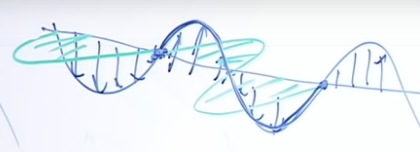
\includegraphics[width=0.9\textwidth]{Wavelength}
\end{figure}

\subsection{Wave/particle duality.}

A photon has energy:
\begin{align*}
	E=&\hslash \omega \text{. Energy of single photon.} \numberthis\label{eq:E_omega}\\
	E_{ray}=&n \hslash \omega \text{. Energy of ray.}
\end{align*}

(I learned quantum mechanics using Planck's constant, $h$, rather than Dirac's $\hbar$; $hf=\hbar\omega$.) 

In modern usage, mass is what used to be called rest mass. $E = m c^2$ only for stationary object.

In particle physics we choose units such that $c=1$ and $\hslash=1$. In this course, $c$ and $\hslash$ will appear explicitly only when Prof. Susskind wants to show the magnitude of some quantity.

Energy depends on the motion of the object as seen by the observer: it isn't a universal thing that everyone will agree on.

Light has energy and momentum (not mass): 

\begin{align*}
	\left|P\right|=&\frac{E}{c} \\
	=&\frac{\hslash \omega}{c} \text{, from (\ref{eq:E_omega})}\\
	=& \frac{2 \pi \hslash}{\lambda} \text{, from (\ref{eq:omega:lambda}). c.f. Harmonic Oscillator.}\numberthis\label{eq:P:lambda}
\end{align*}

This is why we need larger and larger instruments to observe smaller particles!
To see really small things, we need particles with high energy and momentum.


\section{Quantum field theory}

\subsection{Mathematical Preliminaries}

Consider a classical wave $A \sin(kx)$. Energy is proportional to $A^2$, but also to the number of photons, $n$: $E \propto n \hslash \omega$, $A \propto \sqrt{n}$.

Generally, equations containing $c$ apply for photons only. For non-relativistic particles:
\begin{align*}
	E=&\frac{p^2}{2m}\\
	f =& \frac{h}{2 m \lambda^2} \text{. c.f. \Schr equation!}
\end{align*}

\begin{itemize}
	\item Phase Velocity: velocity of wave packet;
	\item Group velocity: velocity of troughs and peaks--identified with particle velocity.
\end{itemize}

For light waves, phase and group velocities are the same, but this isn't true for most particles. Phase velocity can exceed $c$, but it can't transmit information--Section \ref{section:phase:group:velocities}.

Space is infinite. If physics is the art of getting problems into a shape that computers can solve, we need to remove infinities.

Let's look at 1 dimensional waves. In order to get rid of infinities, we can restrict to fixed length $L$: reflecting boundary condition at ends. But this violates conservation of momentum: when wave bounces momentum reverses. Instead use a topological ''circle''\footnote{I.e. we just assume that the ends are connected} circumference $L$--periodic boundary conditions. This gets rid of infinity and preserves conservation of momentum at a cost: momentum is quantized: 

\begin{align*}
	\lambda =& \frac{L}{N} \text{ for some integer $N$}\\
	P =& \frac{h}{\lambda} \text{ allowable momenta}\\
	=& \frac{h N}{L} \numberthis \label{eq:momenta:finit:volume}
\end{align*}

Now make into a real circle, radius $R$, and redefine $L=PR$ to be \emph{angular momentum}.

\begin{align*}
	P =& \frac{h N}{2 \pi R}\\
	L =& N \frac{h}{2 \pi}\\
	=& N \hslash \text{ independent of $R$.}
\end{align*}

\subsection{Quantum field theory}

Start with harmonic oscillator: a wave is a collection of harmonic oscillators. Energy is quantized: 0, $\hslash \omega$, $2\hslash \omega$...

Introduce operators:

\begin{align*}
	a^+ \ket{n} =& \sqrt{n+1} \ket{n+1} \text{, creation operator} \numberthis \label{eq:creation}\\
	a^- \ket{n} =& \sqrt{n} \ket{n-1} \text{, annihilation operator} \numberthis \label{eq:annihilation} \\
	a^+ a^- \ket{n} =& n \ket{n} \text{, or}\\
	a^+ a^-  =& n \text{. Similarly}\\
	a^- a^+  =& n+1\\
	[a^-, a^+] =& 1
\end{align*}

Return to world on a circle--$\omega_N$--equivalent to oscillator. State is $\ket{n_1,n_2, n_3,...}$--occupation numbers. 
\begin{defn}[quantum field]
	A quantum field is a collection of harmonic oscillators, together with annihilation operators and creation operators.
\end{defn}

\section{Quantum fields and particles}

\begin{align*}
	\text{Wave} =& e^{i k x} \text{, $k$ is wave number}\\
	P=&\hslash k\\
	n(k) =& \text{ occupation number.}
\end{align*}

We represent the state of a 1D circular system by occupation numbers, $\ket{...n(-1), n(0), n(1), n(2)...}$, and introduce operators $a^+(k)$, $a^-(k)$. 
\begin{align*}
a^+(1)\ket{...n(-1), n(0), \underbrace{n(1)}_\text{target of $a^+(1)$}, n(2)...}=& \sqrt{n(1)+1}\ket{...n(-1), n(0), n(1)+1, n(2)...}
\end{align*}
$a^+(k)$, $a^-(k)$ are quantum mechanical versions of the Fourier coefficients of a field $\Psi$.

Here is a classical wave:
\begin{align*}
	\Psi(x) =& \sum_k \alpha(k) e^{ikx}\\
	\Psi^*(x) =& \sum_k \alpha^*(k) e^{-ikx}
\end{align*}

We quantize as shown in (\ref{eq:q:1}) and (\ref{eq:q:2}) to produce a quantum field:
\begin{align*}
	\alpha(k) \rightarrow& a^-(k) \numberthis \label{eq:q:1}\\
	\alpha^*(k) \rightarrow& a^+(k) \numberthis \label{eq:q:2}\\
	\Psi(x) =& \sum_k a^-(k) e^{ikx} \numberthis \label{eq:Psi}\\
	\Psi^\dagger(x) =& \sum_k a^+(k) e^{-ikx} \numberthis \label{eq:Psi:dagger}
\end{align*}

We need to justify (\ref{eq:q:1}) and (\ref{eq:q:2}) in some appropriate limit.

How can we describe scattering? Imagine scattering so a particle with momentum $k_7$ becomes a particle with momentum $k_9$: $a^+(k_9)a^-(k_7)\ket{0,0,..1,0,0}$.

What if laws of physics allows number of particles to change? $a^+(k_{16})a^+(k_9)a^-(k_7)\ket{0,0,..1,0,0}$. We can't do this in regular quantum mechanics.

What does $\Psi^\dagger$ do? Start with the vacuum $\ket{0}$.

\begin{align*}
	\Psi^\dagger(x)\ket{0} =& \sum_k a^+(k) e^{-ikx} \ket{0} \text{ from (\ref{eq:Psi:dagger})}\\
	=& \sum_k e^{-ikx} \underbrace{a^+(k) \ket{0}}_\text{One particle state with momentum $k$} \\
	=& \sum_k e^{-ikx} \ket{k} \text{. Superposition gives particle at definite position.}
\end{align*}

If we make the circle larger and larger, $\sum \rightarrow \int$.

What does $\Psi$ do? It annihilates a particle at $x$.

Locality: when something happens, it happens at one spot. Figure \ref{fig:ex:locality} is an example of one particle being replaced by two.

\begin{figure}[H]
	\caption[Example of locality: one particle is replaced by two]{Example of locality: $\Psi^\dagger(x)\Psi^\dagger(x)\Psi(x)\ket{...}$}\label{fig:ex:locality}
	\begin{center}
		\feynmandiagram [horizontal=i1 to a] {
			i1[] -- [fermion,momentum'=\(k\)] a[particle=\(x^{\prime}\)],
			a --[fermion] f1[],
			a--[fermion] f2[],
		};
	\end{center}
\end{figure}



Start with state $\ket{0,...\underbrace{1}_\text{$k_i$},0,000}$.

We assume that $k_i$ denotes the index of the only momentum with a non-zero index.
\begin{align*}
\Psi^\dagger(x)\Psi^\dagger(x)\Psi(x)\ket{0,...1,0,000}=&\sum_m a^+(m) e^{-imx} \sum_l a^+(l) e^{-ilx} \sum_k a^-(k) e^{ikx} \ket{...}\\
=&\sum_m a^+(m) e^{-imx} \sum_l a^+(l) e^{-ilx} a^-(k_i) e^{ik_ix} \ket{...}\\
=&\sum_m a^+(m) e^{-imx} \sum_l a^+(l) e^{-ilx}  e^{ik_ix} \ket{0}\\
=&\sum_{l,m}  e^{-imx}  e^{-ilx}  e^{ik_ix} \underbrace{\ket{001001...}}_\text{$l$ and $m$ are indices of $1s$.}\\
\triangleq &\sum_{l,m}   e^{i(k-l-m)x} \ket{l,m}
\end{align*}

This isn't true if $l=m$! We have two application of $a^+(m)$, so vacuum becomes $\sqrt{2}\ket{...2...}$. Probability of two particles coming out in same state is twice probability of them being in different states.

For the time being we ignore conservation laws!

Consider generating photon at a position where there is a pre-existing photon with momentum $l$--Figure \ref{fig:simple:decay}.
\begin{figure}[H]
	\begin{center}
		\caption[Generating photon  where there is a pre-existing photon]{Generating photon at a position where there is a pre-existing photon with momentum $l$.}\label{fig:simple:decay}
		\feynmandiagram[layered layout,horizontal=in1 to out1]{
			in1--[photon]c--[photon,edge label=\(l\)]out1,
			c--[photon]out2,
		};
	\end{center}
\end{figure}

\begin{align*}
\Psi(x)^\dagger\ket{l} =& \sum_k a^+(k) e^{-ikx} \ket{l}\\
=& \sum_{k\ne l} e^{-ikx} \ket{k,l} + \sqrt{2} e^{-ilx} \ket{l,l}
\end{align*}

Stimulated emission: higher probability of generating particles that are already there (c.f. spontaneous emission). This is true for Bosons, but not Fermions.
 
 Laws for Bosons
 \begin{align*}
 [a^+(k),a^+(l)] =& 0\\
 [a^-(k),a^-(l)] =& 0\\
 [a^-(k),a^+(l)] =& \delta_{k,l}\\
 \Psi(x) =& \sum_k a^-(k) e^{ikx} \\
 \Psi^\dagger(x) =& \sum_k a^+(k) e^{-ikx}
 \end{align*}
 
 \begin{align*}
 \frac{1}{L}\int_\frac{-L}{2}^\frac{L}{2} dx \Psi^\dagger(x) \Psi(x) =& \frac{1}{L} \int_\frac{-L}{2}^\frac{L}{2} dx \sum_k a^+(k) e^{-ikx} \sum_l a^-(l) e^{ilx}\\
 =& \sum_k a^+(k) \sum_l a^-(l) \frac{1}{L} \int_\frac{-L}{2}^\frac{L}{2} e^{-ikx} e^{ilx} dx\\
 =& \sum_k a^+(k) \sum_l a^-(l) \frac{1}{L} \int_\frac{-L}{2}^\frac{L}{2} e^{-i(k-l)x} dx\\
  =& \sum_k a^+(k) \sum_l a^-(l) \delta_{k,l}\\
 =&  \sum_k \underbrace{a^+(k) a^-(k)}_\text{Occupation number}\\
 =& N \text{, total number of particles.}\\
 \Psi^\dagger(x) \Psi(x) =& \text{ density of particles at $x$}.
 \end{align*}


\section{More quantum field theory}

\subsection{Mathematical Preliminaries}

\subsubsection{Dirac Delta function}

\begin{align*}
	\text{For } k =& \frac{2 \pi n}{L}\\
	\int_{-\frac{L}{2}}^{\frac{L}{2}} e^{ikx} dx =& L \text{, if $k =0$}\\
	=& 0 \text{, otherwise}\\
	\rightarrow& 2 \pi \delta(k) \text{ as $k \rightarrow \infty$}
\end{align*}

We will use \emph{ket} vectors for initial states, \emph{bra} for final. This will help with bookkeeping.

\subsubsection{Creation and annihilation operators operating on bra vectors}

\begin{align*}
	\braket{n|m} =& \delta_{n,m}\numberthis \label{eq:orthogonal} \text{. We want the following}\\
	\braket{n|(a^+|m)} =& \braket{(n|a^+)|m}  \numberthis \label{eq:consistency}\\
	=& \sqrt{m+1} \braket{n|m+1} \text{, from (\ref{eq:creation})}\\
	=& \sqrt{m+1} \delta_{n,m+1} \text{, from (\ref{eq:orthogonal})} \text{, so we define}\\
	\bra{n} a^+ \triangleq & \sqrt{n} \bra{n-1} \text{ to satisfy (\ref{eq:consistency}), and} \numberthis \label{eq:bra:create}\\
	\bra{n} a^= \triangleq & \sqrt{n+1} \bra{n-1} \numberthis \label{eq:bra:annihilate}
\end{align*}
Example: calculate an expression two different ways.
\begin{align*}
	\braket{n|(a^+a^-|n)} =& \sqrt{n}\braket{n|(a^+|n-1)}\\
	=& (\sqrt{n})^2 \braket{n|n} \text{ from (\ref{eq:bra:create})}\\
	=& n\\
	\braket{(n|a^+a^-)|n} =& \sqrt{n} \braket{(n-1|a^-)|n}\\
	=& n \braket{n|n} \text{ from (\ref{eq:bra:annihilate})}
\end{align*}

\subsection{Quantum Fields}

The only way we can study particles is to collide them; quantum field theory is the mathematical tool.

We will set $\hslash=1$, so $P=k$, and we will take $X$ and $P$ to be 3 dimensional.
\begin{align*}
\Psi^\dagger(X)(X,t) \triangleq& \sum_k a^+(k) e^{-ikX} e^{i \omega(k) t} \\
\Psi(X)(X,t) \triangleq& \sum_k a^-(k) e^{ikX} e^{- i \omega(k) t}
\end{align*}

\begin{align*}
\omega =& E \text{ and}\\
E =& \frac{P^2}{2m} \text{, whence}\\
\omega =& \frac{k^2}{2m} \numberthis \label{eq:omega:k}
\end{align*}
We  determine the differential equation satisfied by $\Psi^\dagger(X)$.

\begin{align*}
\dot{\Psi^\dagger(X)} =&  \sum_k i \omega(k) a^+(k) e^{-ikX} e^{i \omega(k) t}\\
\frac{\partial^2 \Psi^\dagger(X)}{\partial X^2} =& \sum_k -k^2 a^+(k) e^{-ikX} e^{i \omega(k) t} \numberthis \label{eq:omega:dot}\\
 =& - \sum_k 2m \omega a^+(k) e^{-ikX} e^{i \omega(k) t} \text{ from (\ref{eq:omega:k})}\\
 \frac{1}{2m} \frac{\partial^2 \Psi^\dagger(X)}{\partial X^2} =& - \sum_k \omega a^+(k) e^{-ikX} e^{i \omega(k) t}\\
 =& -\frac{1}{i} \frac{\Psi^\dagger(X)}{\partial t}\\
  i \frac{\Psi^\dagger(X)}{\partial t} =&  \frac{1}{2m} \frac{\partial^2 \Psi^\dagger(X)}{\partial X^2} \text{ From (\ref{eq:omega:dot}). This is \Schr's equation for field!}
\end{align*}

Consider particle scattering from heavy target; we show it conserves energy, but not momentum--Figure \ref{fig:particle:heavy:target}. Assume scattering probability independent of time.

\begin{figure}[H]
	\caption{Particle being absorbed and then re-emitted}\label{fig:particle:heavy:target}
	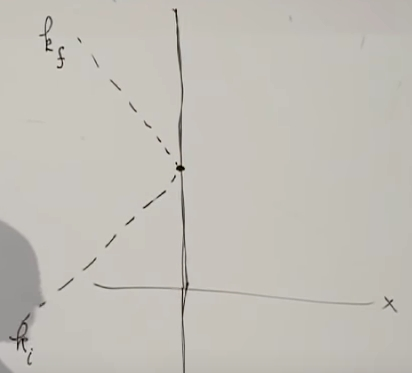
\includegraphics[width=0.8\textwidth]{particle-heavy-target}
\end{figure}

We want the probability of emitting one particle in final state (Introduce coupling constant $g$)--$\big| \bra{k_f} g \int dt \Psi^\dagger(0,t)\Psi(0,t)\ket{k_i} \big|^2$

\begin{align*}
	&\bra{k_f} g \int dt \sum_l \underbrace{a^+(l) e^{i \omega_l t}}_\text{contributes iff $l==k_f$} \sum_k \underbrace{a^-(k) e^{-i \omega_k t} \ket{k_i}}_\text{contributes iff $k==k_i$}\\
	=&\bra{k_f} g \int dt a^+(k_f) e^{i \omega_{k_f} t}  a^-(k_i) e^{-i \omega_{k_i} t} \ket{k_i}\\
	=& g \int dt e^{i(\omega_{k_f}-\omega_{k_i})}\cancel{<0|0>}\\
	=& 2 \pi g \delta(\omega_{k_f}-\omega_{k_i}) \text{--conservation of energy.} \numberthis \label{eq:conservation:energy}
\end{align*}

Conservation of energy works only because of time symmetry!

Probability $\propto g^2$.

Prof. Susskind has shown:
\begin{itemize}
	\item Definition of coupling constant;
	\item Integration over time is the thing that ensures energy conservation;
	\item Scattering amplitude.
\end{itemize}

NB.\begin{itemize}
	\item  If X not zero (say $X_s$), then amplitude gets a phase of $e^{i(k_f-k_i)S_s}$, which doesn't affect probability.
	\item if $g$ is a function of time, it generally means that we are ignoring something.
\end{itemize}

To reiterate: $\Psi$ and $\Psi^\dagger$ are the tools that let us discuss particle interactions.

What if we are dealing with an electron? Each particle has its own $\Psi$. What if one electron goes in but two come out-- $\Psi^\dagger(0,t)\Psi^\dagger(0,t)\Psi(0,t)$? Or two in, two out--$\Psi^\dagger(0,t)\Psi^\dagger(0,t)\Psi(0,t)\Psi(0,t)$? Which are allowed? One rule is that there must be the same number of $\Psi^\dagger$s and $\Psi$s. Imagine multiplying by a phase:

\begin{align*}
\Psi \rightarrow & e^{i\alpha} \Psi \numberthis \label{eq:conservation:charge1}\\
\Psi^\dagger \rightarrow & e^{-i\alpha} \Psi^\dagger \numberthis \label{eq:conservation:charge2}
\end{align*}

Allowable combinations are invariant under multiplication by $e^{i\alpha}$--charge is conserved. Table \ref{table:conserve} shows some pairs of symmetries and conservation laws.

\begin{table}[H]
	\caption{Invariance and Conservation Laws}\label{table:conserve}
	\begin{center}
			\begin{tabular}{|l|l|l|}  \hline
				Invariance&Conservation&Ref\\ \hline
				Time& Energy&(\ref{eq:conservation:energy})\\  \hline
				Space&Charge&(\ref{eq:conservation:charge1}),  (\ref{eq:conservation:charge2})\\ \hline
				Phase&Momentum&Section \ref{sec:momentum:conservation}\\ \hline
			\end{tabular}
	\end{center}
\end{table}

NB, this isn't a real electron, as $\Psi$ is for Bosons. A negative pion would be OK.


\section{Energy conservation and waves}\label{sec:energy:conservation}

\subsection{Phase Velocity and Group Velocity}\label{section:phase:group:velocities}

\subsubsection{Phase Velocity and Group Velocity of non-relativistic particles}
Generally phase velocity doesn't have anything to do with measurable things in quantum mechanics. Group velocity is what counts.

Consider $\sin(kx-\omega t)$. The wave moves so that $kx-\omega t$ remains constant.
\begin{align*}
	x =& \underbrace{\frac{\omega}{k}}_{\mathclap{\substack{\text{phase }\\
															\text{velocity}}}} t\\
	\omega =& \frac{2 \pi}{T}\\
	k =& \frac{2 \pi}{\lambda}
\end{align*}

This is connected with the \Schr equation, since $\omega$ is energy, and $k$ momentum, so:
\begin{align*}
	\omega=&\frac{k^2}{2m} \text{, whence} \numberthis \label{fig:phase:c}\\
	\frac{\omega}{k}=&\frac{k}{2m} \text{, phase velocity.}\\
	=& \frac{v}{2}  \text{, where $v$ is velocity of classical particle.}
\end{align*}
 Let's add a constant to frequency, hence to the energy:
\begin{align*}
	\omega=&\frac{k^2}{2m}+c 
\end{align*}
Adding $c$ changes the phase velocity--but changing $E$ by an additive constant has no physical effect! Now we write:
\begin{align*}
	\Psi =& \sum_k a^-(k) e^{ikx}e^{- i \omega(k) t} e^{-i c t}
\end{align*}
Given a solution to the \Schr equation, adding a constant to the phase just multiplies $\Psi$ by $e^{-i c t}$. All of the quantities of physical interest that are made out of the \Schr field involve $\Psi\Psi^\dagger=\cancel{e^{-i c t}}\Psi \cancel{e^{+i c t}}\Psi^\dagger$: e.g. probability density, expectation values. There is no physical sense to adding a constant, but it does change the phase velocity. We see that the phase velocity isn't measurable; it is an artifact of the mathematics. On the other hand, the group velocity does mean something.

Given a bunch of plain waves, how can we get them to add up to a concentrated lump? (Which will turn out to move with something called the group velocity.) The answer is destructive interference: the waves add someplace, and cancel out in other places. If we have a bunch of waves, and are interested in how the waves of slightly different frequency reinforce each other, let's look at two waves, whose momenta are close, and try to see how it all works. We will try to follow where the constructive interference takes place between two waves.

\begin{align*}
	\sin(kx-\omega(k)t) +& \sin(k^\prime x-\omega(k^\prime)t)\text{ will reinforce each other when}\\
	kx-\omega(k)t=&k^\prime x-\omega(k^\prime)t\text{, i.e. when}\\
	x =& \frac{\omega-\omega^\prime}{k-k^\prime}t\\
	\rightarrow & \underbrace{\frac{d \omega}{dk}}_{\mathclap{\substack{\text{group  }\\
	\text{velocity}}}} t \text{, as $k-k^\prime \rightarrow 0$}
\end{align*}
The point where the waves reinforce each other will travel with the \emph{group velocity}:
\begin{align*}
	V_g\triangleq&\frac{d \omega}{dk}\\
	=&\frac{k}{m} \text{, from \eqref{fig:phase:c}}
\end{align*}
\begin{itemize}
	\item The group velocity does not depend on $c$
	\item The group velocity matches the velocity of a non-relativistic particle.
\end{itemize}

\subsubsection{Phase Velocity and Group Velocity of Relativistic Particles}

We will calculate the phase velocity and group velocity  of a relativistic particle, starting with the relationship between energy and momentum. 

\begin{align*}
	E =& \sqrt{P^2 + m^2} \text{, which leads to the wave equation}\\
	\omega =& \sqrt{k^2 + m^2}
\end{align*}
At speed of light(m=0), so
\begin{align*}
	\omega =& \left| k \right|\\
	V_p =& \frac{\omega}{k} \text{ phase velocity of photon waves}\\
	 =&1\\
	 V_g =& \frac{d\omega}{dk} \text{ group velocity of photon waves}\\
	 =&1
\end{align*}
So the group velocity and phase velocity are the same for a massless particle. Now lets us make $m>0$
\begin{align*}
	V_p =& \frac{\omega}{k}\\
	=&\sqrt{\frac{k^2+m^2}{k^2}}\\
	=&\sqrt{1+\frac{m^2}{k^2}} \numberthis \label{eq:rel:phase:V}\\
	>&1
\end{align*}
\begin{align*}
	V_g =& \frac{d\omega}{dk} \\
	=& \frac{\cancel{2}k}{\cancel{2}\sqrt{k^2+m^2}}\\
	=& \frac{1}{\sqrt{1+\frac{m^2}{k^2}}} \numberthis \label{eq:rel:group:V}\\
	<&1 \text{. Combining \eqref{eq:rel:phase:V} and \eqref{eq:rel:group:V}}\\
	V_p V_g =& 1
\end{align*}

If $\omega\propto k$, the waves all have the same phase and group velocities irregardless of frequency: the difference between group and phase velocities is connected to dispersion.

\subsection{Momentum Conservation}\label{sec:momentum:conservation}

In the discussion around Figure \ref{fig:particle:heavy:target}, leading to \eqref{eq:conservation:energy}, we saw how time invariance led to the conservation of energy. We integrated over all possible times; because the process could happen at any time:
\begin{align*}
	&\bra{k_f}  \int dt a^+(k_f) e^{i \omega_{k_f} t}  a^-(k_i) e^{-i \omega_{k_i} t} \ket{k_i}\\
	=&  \int dt e^{i(\omega_{k_f}-\omega_{k_i})}\cancel{<0|0>}\\
	=& 2 \pi  \delta(\omega_{k_f}-\omega_{k_i})
\end{align*}
Now we will show how a process that can occur anywhere in space leads to conservation of momentum.  Figure \ref{fig:split:particle} shows a particle splitting into two particles. 
 
\begin{figure}[H]
	\begin{center}
		\caption[Split Particle at any position $x$]{Split Particle at any position $x$. A particles is eaten at $x$, and two particles are created at the same point: $\bra{k_1^\prime,k_2^\prime}\int \Psi^\dagger(x)\Psi^\dagger(x)\.\Psi(x) dx\ket{k}$}\label{fig:split:particle}
		\feynmandiagram[horizontal'=out1 to out2]{
			in1--[fermion, edge label=\(k\)]c--[fermion, edge label=\(k_1\)]out1,
			c--[fermion, edge label=\(k_2\)]out2,
		};
	\end{center}
\end{figure}

\begin{align*}
	\bra{k_1^\prime,k_2^\prime}&\int \Psi^\dagger(x)\Psi^\dagger(x)\Psi(x) dx\ket{k}\\
	=&\bra{k_1^\prime,k_2^\prime}\int \underbrace{a^+(k_1^\prime) a^+(k_2^\prime)}_{\mathclap{\substack{\text{Create 2}\\
		\text{particles}}}} \underbrace{a^-(k)}_\text{Eat particle} \underbrace{e^{ikx} e^{-i(k_1^\prime+k_2^\prime)x}}_{\mathclap{\substack{\text{integrates to }\\
	\text{Dirac-$\delta$--(\ref{eq:conservation:energy})}}}} dx\ket{k}
\end{align*}

So invariance under space translation yields conservation of momentum.

Another \emph{possible} symmetry: $\Psi \rightarrow e^{i \lambda} \Psi$. There is no change to probabilities if number of $\Psi$s is same as number of $\Psi^\dagger$s. This is connected with conservation of charge.

\subsection{Fermions}

\subsubsection{Introduction to Fermions}

\begin{itemize}
	\item Can have any number of Bosons in any state (same place);
	\item Bosons have a tendency to accumulate in the same state. E.g. consider a particle that decays and emits a photon. If lots of other photons already on some state, decay will preferentially favour that state.
\end{itemize}

Fermions cannot be in same state (Pauli Exclusion Principle). We will start the same way we did with Bosons.

\begin{align*}
	\Psi(x) =& \sum_k a^-(k) e^{ikx}
\end{align*}
The state of the system is once again a vector showing the number of particles in each state, but these numbers can be $0$ or $1$ only because of the Pauli exclusion principle: $\ket{001...01010...}$. Again we have:
\begin{align*}
	\Psi^\dagger(x) =& \sum_k a^+(k) e^{-ikx}
\end{align*}

Focus on one state, either full $(\ket{1})$ or empty $(\ket{0})$: those are only two possibilities. What are the algebraic rules for creation and annihilation operators?

\begin{align*}
	c^+\ket{0} =& \ket{1} \text{, for Fermions use $c$ rather than $a$}\\
	c^+\ket{1} =& 0 \text{, i.e. $\psi(x) \equiv 0$}\\
	c^-\ket{1} =& \ket{0}\\
	c^-\ket{0} =& 0\\
\end{align*}

We deduce:
\begin{align*}
	c^+c^-\ket{0} =& 0\\
	c^-c^+\ket{0} =& \ket{0}\\
	(c^+c^-+c^-c^+)\ket{0} =& \ket{0}\\
	c^+c^-\ket{1} =& \ket{1} \\
	c^-c^+\ket{1} =&0 \\
	(c^+c^-+c^-c^+)\ket{1} =& \ket{1}
\end{align*}
We define the anticommutator:
\begin{align*}
	\{c^+,c^-\} \triangleq& (c^+c^-+c^-c^+) \text{, then}\\
	\{c^+,c^-\} =& 1\\
	\{c^+,c^+\} =&0 \\
	\{c^-,c^-\} =&0
\end{align*}
So Fermions have parallel mathematics to Bosons: $[,] \leftrightarrow \{,\}$. We cannot put two particles into the same state, as $c^+c^+=0$.

What about different momenta? We can show that:
\begin{align*}
	\{c^+_k,c^-_{k^\prime} \} =& \delta_{k,k^\prime} \\
	\{c^+_k,c^+_{k^\prime} \} =&0 \\
	\{c^-_k,c^-_{k^\prime} \} =&0
\end{align*}

This shows we can't put two Fermions into the same momentum state. Can we have two Fermions at the same position? Let's try to create them at the origin.

\begin{align*}
	\Psi^\dagger(0) \Psi^\dagger(0) \ket{0} =& \sum_{k,k^\prime} c^+_k c^+_{k^\prime} \ket{0}\\
	==& \frac{1}{2} \sum_{k,k^\prime} \{c^+_k, c^+_{k^\prime}\} \ket{0}\\
	=& 0
\end{align*}

So the answer is no: we can't have two Fermions in the same quantum state (e.g. momentum and spin). So we can't have an electron laser.

There was a question about whether two electrons in two different hydrogen atoms can have the same momentum. LS explained that the electrons are in energy states (not momentum), and each has a separate wave function. They are distinguishable by position.

A system is a collection of degrees of freedom. In classical mechanics, a state is a a set of values for the degrees of freedom; in \glsdesc{gls:QM} a state is everything you have to specify to encompass everything that can be measured.

\subsubsection{Ground State}
We now compare the ground state of a system of Bosons with the ground state of a system of Fermions. In Figure \ref{fig:electons:confined:momentum} we have some particles confined in momentum space. If particles are confined to be within a given volume, then momenta are discrete--\eqref{eq:momenta:finit:volume}. The same thing happens if the momenta are confined.

\begin{figure}[H]
	\begin{center}
		\caption[Particles confined in momentum space]{Allowable momenta of particles confined in periodic 3 dimensional box in momentum space}\label{fig:electons:confined:momentum}
		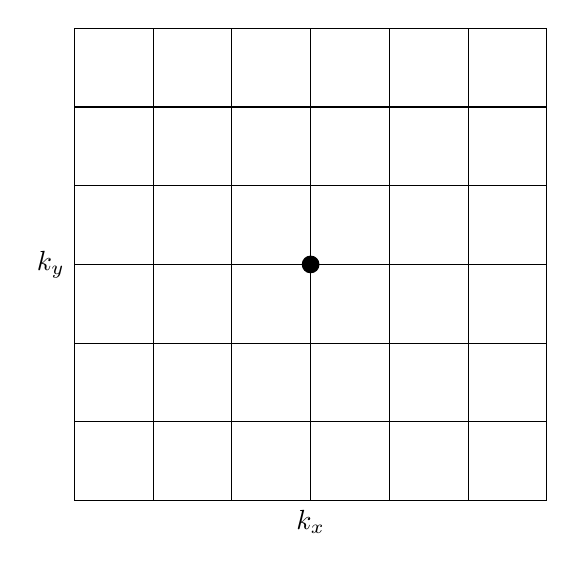
\begin{tikzpicture}
			\draw(0,0)--(0,6)--(6,6)--(6,0)--(0,0);
			\draw(1,0)--(1,6);
			\draw(2,0)--(2,6);
			\draw(3,0)--(3,6);
			\draw(4,0)--(4,6);
			\draw(5,0)--(5,6);
			\draw (6,1)--(0,1);
			\draw (6,2)--(0,2);
			\draw (6,3)--(0,3);
			\draw (6,4)--(0,4);
			\draw (6,5)--(0,5);
			\filldraw[black] (3,3) circle (3pt);
			\node[anchor=east] at (0,3) {$k_y$};
			\node[anchor=north] at (3,0) {$k_x$};
		\end{tikzpicture}
	\end{center}
\end{figure}

Let us take $N$ bosons, and put them into our box. Start with an empty box, and put one boson in. It will go to the state with lowest energy, zero momentum: $\frac{p^2}{m}=0$. Add another boson, in the same place, then another. We can put all $N$ bosons into the same momentum state, giving a \gls{gls:bose:conensate}. The wave function fills the box, and is uncertain about position.


This is very different from what happens with Fermions. Let us try adding Fermions, ignoring spin, each one going into the lowest energy state. We can add the first one in the zero momentum state, as in Figure \ref{fig:electons:confined:momentum}. Once we have filled that state, the next Fermion has to go into the next higher energy level--Figure \ref{fig:electons:lowest:energy}. We can continue, but after 5 electrons have been added (2 dimensional case, 7 for 3 dimensional) the level will be full--Figure \ref{fig:electons:lowest:energy:filled}. Continuing, we want to add electrons to the smallest sphere hat we can--Figure \ref{fig:electons:crowd:into:sphere}. This will have a lot more energy than the corresponding Boson system. Moreover, the electrons will fill a sphere in momentum space, whose boundary depends on the number of electrons--the \gls{gls:fermi:sphere}. 

\begin{figure}[H]
	\caption{Adding more Fermions}\label{fig:adding:more:fermions}
	\begin{subfigure}{0.32\textwidth}
		\caption{Two electrons, lowest possible energy}\label{fig:electons:lowest:energy}
		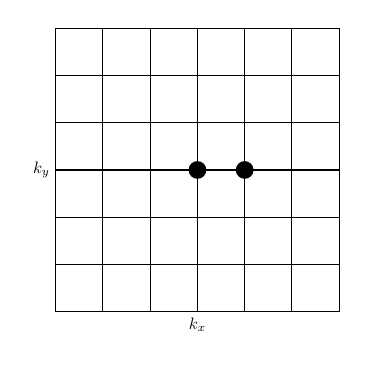
\begin{tikzpicture}[scale=0.6, transform shape]
			\draw(0,0)--(0,6)--(6,6)--(6,0)--(0,0);
			\draw(1,0)--(1,6);
			\draw(2,0)--(2,6);
			\draw(3,0)--(3,6);
			\draw(4,0)--(4,6);
			\draw(5,0)--(5,6);
			\draw (6,1)--(0,1);
			\draw (6,2)--(0,2);
			\draw (6,3)--(0,3);
			\draw (6,4)--(0,4);
			\draw (6,5)--(0,5);
			\filldraw[black] (3,3) circle (5pt);
			\filldraw[black] (4,3) circle (5pt);
			\node[anchor=east] at (0,3) {$k_y$};
			\node[anchor=north] at (3,0) {$k_x$};
		\end{tikzpicture}
	\end{subfigure}
	\hfill
	\begin{subfigure}{0.32\textwidth}
		\caption{Filled lowest two energy levels. The arrow indicates where a particle might go in the third energy level.}\label{fig:electons:lowest:energy:filled}
		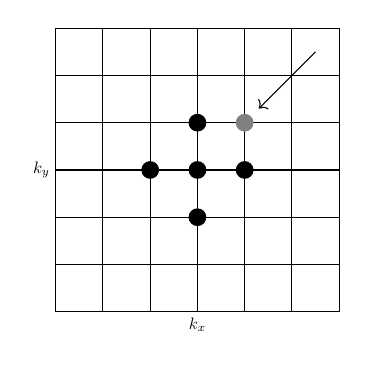
\begin{tikzpicture}[scale=0.6, transform shape]
			\draw(0,0)--(0,6)--(6,6)--(6,0)--(0,0);
			\draw(1,0)--(1,6);
			\draw(2,0)--(2,6);
			\draw(3,0)--(3,6);
			\draw(4,0)--(4,6);
			\draw(5,0)--(5,6);
			\draw (6,1)--(0,1);
			\draw (6,2)--(0,2);
			\draw (6,3)--(0,3);
			\draw (6,4)--(0,4);
			\draw (6,5)--(0,5);
			\filldraw[black] (3,3) circle (5pt);
			\filldraw[black] (4,3) circle (5pt);
			\filldraw[black] (2,3) circle (5pt);
			\filldraw[black] (3,2) circle (5pt);
			\filldraw[black] (3,4) circle (5pt);
			\filldraw[gray] (4,4) circle (5pt);
			\draw[->] (5.5,5.5)--(4.3,4.3);
			\node[anchor=east] at (0,3) {$k_y$};
			\node[anchor=north] at (3,0) {$k_x$};
		\end{tikzpicture}
	\end{subfigure}
	\hfill
	\begin{subfigure}{0.32\textwidth}
		\caption{$E=\frac{k^2}{2m}$, so there are more positions in each energy level as energy increases.}\label{fig:electons:crowd:into:sphere}
		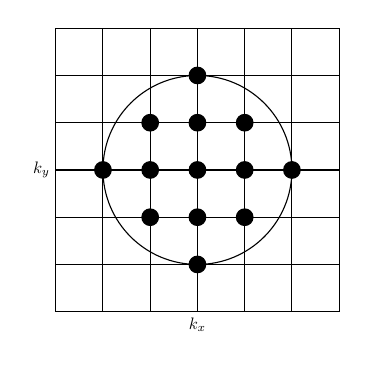
\begin{tikzpicture}[scale=0.6, transform shape]
			\draw(0,0)--(0,6)--(6,6)--(6,0)--(0,0);
			\draw(1,0)--(1,6);
			\draw(2,0)--(2,6);
			\draw(3,0)--(3,6);
			\draw(4,0)--(4,6);
			\draw(5,0)--(5,6);
			\draw (6,1)--(0,1);
			\draw (6,2)--(0,2);
			\draw (6,3)--(0,3);
			\draw (6,4)--(0,4);
			\draw (6,5)--(0,5);
			\filldraw[black] (3,3) circle (5pt);
			\filldraw[black] (4,3) circle (5pt);
			\filldraw[black] (2,3) circle (5pt);
			\filldraw[black] (3,2) circle (5pt);
			\filldraw[black] (3,4) circle (5pt);
			\filldraw[black] (5,3) circle (5pt);
			\filldraw[black] (1,3) circle (5pt);
			\filldraw[black] (3,1) circle (5pt);
			\filldraw[black] (3,5) circle (5pt);
			\filldraw[black] (4,4) circle (5pt);
			\filldraw[black] (2,2) circle (5pt);
			\filldraw[black] (2,4) circle (5pt);
			\filldraw[black] (4,2) circle (5pt);
			\draw(3,3) circle(2.0);
			\node[anchor=east] at (0,3) {$k_y$};
			\node[anchor=north] at (3,0) {$k_x$};
		\end{tikzpicture}
	\end{subfigure}
\end{figure}

We can move Bosons and Fermions out of the ground state, as shown in Figures \ref{fig:bosons:move:ground:state} and \ref{fig:fermions:move:ground:state}.
\begin{figure}[H]
	\caption[Moving Bosons and Fermions from lowest state]{Moving Bosons and Fermions from lowest state. We can think of  (\subref{fig:fermions:move:ground:state}) and (\subref{fig:fermi:surface}) as a low energy photon being absorbed by an electron,knocking it out and leaving a hole, or a photon annihilating to create an electron and a hole. }
	\begin{subfigure}[t]{0.45\textwidth}
		\caption{Initially the Bosons are all in the Ground State. Then we move one up to the first excited state. Which one? It doesn't matter for Bosons.}\label{fig:bosons:move:ground:state}
		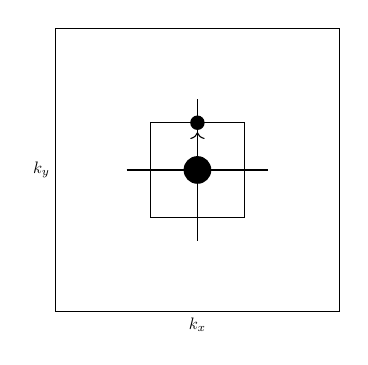
\begin{tikzpicture}[scale=0.6, transform shape]
			\draw(0,0)--(0,6)--(6,6)--(6,0)--(0,0);
			\draw(1.5,3)--(4.5,3);
			\draw(3,1.5)--(3,4.5);
			\draw(4,2)--(2,2)--(2,4)--(4,4)--(4,2);
			\filldraw[black] (3,4) circle (4pt);
			\filldraw[black] (3,3) circle (8pt);
			\draw[->](3,3)--(3,3.8);
			\node[anchor=east] at (0,3) {$k_y$};
			\node[anchor=north] at (3,0) {$k_x$};
		\end{tikzpicture}
	\end{subfigure}
	\hfill
	\begin{subfigure}[t]{0.45\textwidth}
		\caption{Moving Fermions to an excited state. It would not be a good idea to move an electron from deep inside the \gls{gls:fermi:sphere} as it would requires a lot of energy. (We can't move it within \gls{gls:fermi:sphere}, as we are dealing with Fermions.)}\label{fig:fermions:move:ground:state}
		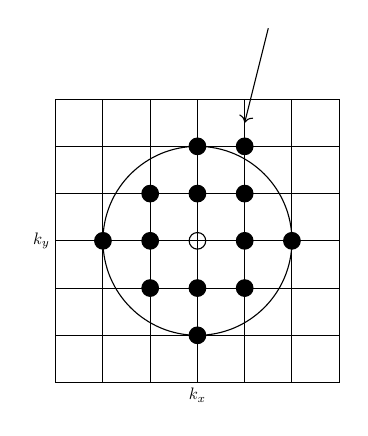
\begin{tikzpicture}[scale=0.6, transform shape]
			\draw(0,0)--(0,6)--(6,6)--(6,0)--(0,0);
			\draw(1,0)--(1,6);
			\draw(2,0)--(2,6);
			\draw(3,0)--(3,6);
			\draw(4,0)--(4,6);
			\draw(5,0)--(5,6);
			\draw (6,1)--(0,1);
			\draw (6,2)--(0,2);
			\draw (6,3)--(0,3);
			\draw (6,4)--(0,4);
			\draw (6,5)--(0,5);
			\draw (3,3) circle (5pt);
			\filldraw[black] (4,3) circle (5pt);
			\filldraw[black] (2,3) circle (5pt);
			\filldraw[black] (3,2) circle (5pt);
			\filldraw[black] (3,4) circle (5pt);
			\filldraw[black] (5,3) circle (5pt);
			\filldraw[black] (1,3) circle (5pt);
			\filldraw[black] (3,1) circle (5pt);
			\filldraw[black] (3,5) circle (5pt);
			\filldraw[black] (4,4) circle (5pt);
			\filldraw[black] (2,2) circle (5pt);
			\filldraw[black] (2,4) circle (5pt);
			\filldraw[black] (4,2) circle (5pt);
			\draw(3,3) circle(2.0);
			\filldraw[black](4,5) circle(5pt);
			\draw[->](4.5,7.5)--(4,5.5);
			\node[anchor=east] at (0,3) {$k_y$};
			\node[anchor=north] at (3,0) {$k_x$};
		\end{tikzpicture}
	\end{subfigure}
	\begin{subfigure}[t]{0.45\textwidth}
		\caption{Instead we take from near the surface of \gls{gls:fermi:sphere} to minimize energy required. This creates an electron with a little bit of energy above the \gls{gls:fermi:sphere}, but it also leaves a hole. Imagine a box full of positive charge, plus enough electrons to fill the \gls{gls:fermi:sphere} (The \gls{gls:fermi:sea}). It's electrically neutral, as the numbers of electrons and protons are equal. When we move an electron we have a little bit of energy above the \gls{gls:fermi:surface}, and a hole where the particle is missing: it can be thought of as a positive charged particle.}\label{fig:fermi:surface}
		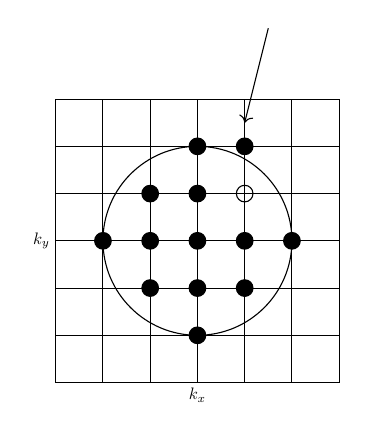
\begin{tikzpicture}[scale=0.6, transform shape]
			\draw(0,0)--(0,6)--(6,6)--(6,0)--(0,0);
			\draw(1,0)--(1,6);
			\draw(2,0)--(2,6);
			\draw(3,0)--(3,6);
			\draw(4,0)--(4,6);
			\draw(5,0)--(5,6);
			\draw (6,1)--(0,1);
			\draw (6,2)--(0,2);
			\draw (6,3)--(0,3);
			\draw (6,4)--(0,4);
			\draw (6,5)--(0,5);
			\filldraw[black] (3,3) circle (5pt);
			\filldraw[black] (4,3) circle (5pt);
			\filldraw[black] (2,3) circle (5pt);
			\filldraw[black] (3,2) circle (5pt);
			\filldraw[black] (3,4) circle (5pt);
			\filldraw[black] (5,3) circle (5pt);
			\filldraw[black] (1,3) circle (5pt);
			\filldraw[black] (3,1) circle (5pt);
			\filldraw[black] (3,5) circle (5pt);
			\draw[black] (4,4) circle (5pt);
			\filldraw[black] (2,2) circle (5pt);
			\filldraw[black] (2,4) circle (5pt);
			\filldraw[black] (4,2) circle (5pt);
			\draw(3,3) circle(2.0);
			\filldraw[black](4,5) circle(5pt);
			\draw[->](4.5,7.5)--(4,5.5);
			\node[anchor=east] at (0,3) {$k_y$};
			\node[anchor=north] at (3,0) {$k_x$};
		\end{tikzpicture}
	\end{subfigure}
	\hfill
	\begin{subfigure}[t]{0.45\textwidth}
		\caption{Energy required to move an electron from just below \gls{gls:fermi:surface} to above. We need a little bit of energy to move to the surface from below, plus a little to move to position above. We an think of the second as the energy of the electron, and the first as the energy of the hole. The electron might move around, and then suddenly pop into the hole, emitting a photon that takes away the extra energy. The hole is a fake particle with the opposite charge to an electron. It can come together with the electron and annihilate.}
		\begin{tikzpicture}[scale=0.6, transform shape]
			\draw (-5,0) to (5,0) node[anchor=east]{Fermi Surface};
			\filldraw[black] (3,2) circle (5pt);
			\draw(-1,-2) circle(5pt);
			\draw[->] (-1,-2) to (-1,-0.2);
			\draw[->] (-1,0) to (2.8,1.8);
		\end{tikzpicture}
	\end{subfigure}
\end{figure}

In Figure \ref{fig:fermions:move:ground:state} a charged hole is left behind.
If an electron drops into hole, a photon is emitted.

Consider an atom, with all electrons in their ground state. Low energy electron is struck by photon, which takes electron to excited state.

Electrons that are deep in \gls{gls:fermi:sea} can't be excited by low energy photons. Only shallow electrons are accessible.

\subsubsection{Dirac and antiparticles}

We start with the 1-dimensional case. Imagine a wave propagating to the right with speed $c$.
\begin{align*}
	\omega =& k\\
	\frac{\partial \psi}{\partial t} =& - \frac{\partial \psi}{\partial x}  \numberthis \label{eq:rh:dirac}\\
	\psi =& e^{i(kx-\omega t)} \numberthis \label{eq:rh:dirac:wave}
\end{align*}

What if $k$ negative? Then we have negative energy. But if we had arbitrarily negative energies, particle could keep emitting photons all the way down. So (\ref{eq:rh:dirac}) would not make sense for Fermions.

Dirac said to pretend that all the negative energy states were filled, just like filling the \gls{gls:fermi:sphere}: that is the lowest energy state, i.e. the \emph{vacuum}. Now we can take an electron out, leaving a hole. We then have two positive energy objects, electron and positron.( This only makes sense for Bosons, only Fermions). There are some things wrong with this electron:
\begin{itemize}
	\item it only moves to the right;
	\item it moves at the speed of light.
\end{itemize}

\section{The Dirac equation and the Higgs particles}

\subsection{The Dirac equation}

The simplest version of the Dirac Equation  (\ref{eq:rh:dirac}), applies to both electrons and positrons, provided they are moving to the right. We will start with the following equation:
\begin{align*}
	\psi_R =& e^{i(kx-\omega t)} \text{The group velocity is:} \numberthis \label{eq:rh:dirac:wave1}\\
	V_g =& \frac{\omega}{k} \text{, assuming the relationship between $k$ and $\omega$ is linear.}
\end{align*}

If $V_g>0$ the wave moves to the right, otherwise it moves to the left.

Now, we write down another equation, c.f. \eqref{eq:rh:dirac}:
\begin{align*}
	\frac{\partial \psi_R}{\partial t} + \frac{\partial \psi_R}{\partial x} =&0 \text{. This has the solution \eqref{eq:rh:dirac:wave1}}, provided:\\
	\omega =& k
\end{align*}
If $k<0$, $\omega<0$, i.e. negative energy, which is not a good thing: electrons would not be stable. So we fill up the \gls{gls:dirac:sea}, so all negative energy states are filled. Then we can remove one electron, creating a hole in the \gls{gls:dirac:sea}; particle and hole both have positive momentum and positive energy.

We now introduce left moving electrons.

\begin{align*}
	\frac{\partial \psi_L}{\partial t} =& \frac{\partial \psi_L}{\partial x} \numberthis \label{eq:lh:dirac:wave}\\
	\frac{\omega}{k} =& -1
\end{align*}
Fill sea with left moving negative energy.

Define $\psi=\begin{pmatrix}
	\psi_R\\
	\psi_L
\end{pmatrix}$, and write (\ref{eq:rh:dirac:wave}) and (\ref{eq:lh:dirac:wave}):

\begin{align*}
	\frac{\partial \psi}{\partial t} =& - \alpha \frac{\partial \psi}{\partial x} \text{, where}\\
	\alpha =& \begin{pmatrix}
		1&0\\
		0&-1
	\end{pmatrix} \text{. We will find the following useful:} \numberthis\label{eq:alpha}\\
	\omega =& \alpha k \numberthis \label{eq:dirac:1}
\end{align*}

Now we give the particles mass $m$.
\begin{align*}
	\omega^2 =& k^2 + m^2 \text{. Now we generalize (\ref{eq:dirac:1})} \numberthis \label{eq:omega:relativistic}\\
	\omega =& \alpha k + m \beta  \numberthis \label{eq:Dirac:1D}
\end{align*}
This is the 1D Dirac equation, which gives:
\begin{align*}
	\omega^2 =& \alpha^2 k^2 + m^2 \beta^2 + m k (\alpha \beta + \beta \alpha) \text{, which agrees with \eqref{eq:omega:relativistic} iff:}\\
	\alpha^2 =& 1 \text{, already satisfied by (\ref{eq:alpha})}\\
	\beta^2 =& 1 \text{, and}\numberthis \label{eq:beta2}\\ 
	\{\alpha,\beta\} =& 0 \numberthis \label{eq:alpha:beta}\\
	\beta =& \begin{pmatrix}
	0 & 1\\
	1 & 0
	\end{pmatrix} \text{ satisfies (\ref{eq:beta2}) and (\ref{eq:alpha:beta}).}
\end{align*}

The mass term couples equations for $\Psi_L$ and $\Psi_R$. The Dirac equation is Lorentz covariant.

Let us make particle stand still, i.e. $k=0 \implies \omega = \beta m$.

\begin{align*}
	i \frac{\partial \psi}{\partial t} =& \beta m \Psi\\
	i \dot{\psi_R} =& m \psi_L\\
	i \dot{\psi_L} =&  m \psi_R \\
	i \dot{\psi_+} =&  m \psi_+ \text{, where $\psi_+\triangleq\psi_R + \psi_L$--corresponds to $\omega=m$}\\
	i \dot{\psi_-} =&  m \psi_- \text{, where $\psi_-\triangleq\psi_R - \psi_L$--corresponds to $\omega=-m$}
\end{align*}

So particle at rest still has positive and negative energies: throw latter in Dirac Sea.

\subsection{Higgs particles}

In the presence of the Higgs field, $\phi(x)$, the Dirac equation becomes:
\begin{align*}
	i \dot{\psi_R} =& -i \partial_x \psi_R + g \phi \psi_L\\
	i \dot{\psi_L} =& i \partial_x \psi_L + g \phi \psi_R \text{, which gives massless electron if $\phi=0$}
\end{align*}
What if the lowest energy of Higgs favours a non-zero value, $\phi(x)=\phi$? The $m=g\phi$. This could come about as the result of non-lienar interactions between Boson and Fermions.

The Higgs field is a Bosonic field, which has an energy from a potential, $V(\phi)$. There is a symmetry so $V(\phi)=V(-\phi)$.

\begin{figure}[H]
	\caption[Higgs potential]{Higgs potential: reason for shape not fully understood at time of lecture.}
	\begin{subfigure}{0.5\textwidth}
		\caption{Higgs potential, showing two minima. Either one gives rise to mass of $g\phi$}\label{fig:higgs:potential}
		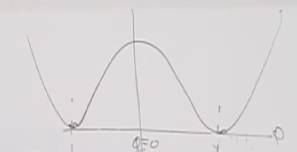
\includegraphics[width=0.8\textwidth]{higgs-potential}
	\end{subfigure}
	\begin{subfigure}{0.5\textwidth}
		\caption{Higgs field vibrating around vacuum. Frequency is related to mass of Higgs particle: Higgs corresponds to quanta of vibration.}
		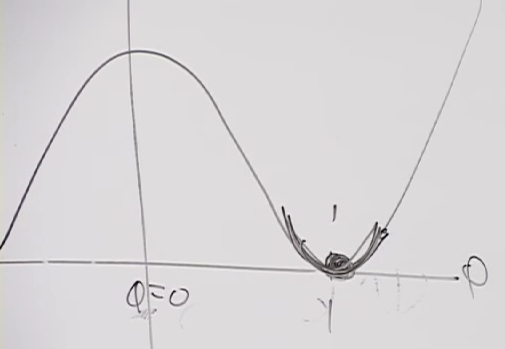
\includegraphics[width=0.8\textwidth]{higgs-vibrating}
	\end{subfigure}
\end{figure}

If Higgs field is coupled in an interesting way to Fermions, Higgs will respond to collisions of Fermions and create Higgs particles. In the Standard Model there is only one Higgs, Supersymmetry has two.

If vacuum were symmetric--Figure \ref{fig:higgs:potential}-- $\phi$ would be zero: it is the breaking of the symmetry which gives electron its mass. All particles except photon get their mass through the Higgs Mechanism. Except for Higgs particle: it gets its mass from a different mechanism.

\subsection{3+1 Dimensional Dirac Equation}

Dirac started with a generalization of \eqref{eq:Dirac:1D}:

\begin{align*}
	\omega =& \underbrace{\alpha . k}_{\alpha_1 k_1 + \alpha_2 k_2 + \alpha_3 k_3} +\beta m\\
	=& \alpha_1 k_1 + \alpha_2 k_2 + \alpha_3 k_3 +\beta m \numberthis \label{eq:omega:3D}\\
\end{align*}
In 3 dimensions, \eqref{eq:omega:relativistic} generalizes to:
\begin{align*}
	\omega^2 =& k_1^2 + k_2^2 +k_3^2 +m^2 \text{, but \eqref{eq:omega:3D} gives}\\
	=& (\alpha_1 k_1 + \alpha_2 k_2 + \alpha_3 k_3 +\beta m)(\alpha_1 k_1 + \alpha_2 k_2 + \alpha_3 k_3 +\beta m)
\end{align*}
These expressions agree iff:
\begin{align*}
	\alpha_i^2 =& 1  \text{ and} \numberthis \label{eq:dirac:ac1}\\
	\beta^2 =& 1 \text{ and} \numberthis \label{eq:dirac:ac2}\\
	\{\alpha_i,\alpha_j\} =& 2 \delta_{i,j} \numberthis \label{eq:dirac:ac3}\\
	\{\alpha_i,\beta\} =& 0 \numberthis \label{eq:dirac:ac4}
\end{align*}

Theorem \ref{thm:dirac:anticommutation} shows 2 or 3 dimensional matrices cannot satisfy these equations; $4 \times 4$ is the first case.

Here is a set of Dirac Matrices (not unique, but equivalent--Theorem \ref{thm:dirac:anticommutation} presents a different set).

\begin{align*}
	\beta =& \begin{pmatrix}
		1&0&0&0\\
		0&1&0&0\\
		0&0&-1&0\\
		0&0&0&-1
	\end{pmatrix} \numberthis \label{eq:beta:1}\\
	\alpha_1 =& \begin{pmatrix}
		0&0&0&1\\
		0&0&1&0\\
		0&1&0&0\\
		1&0&0&0
	\end{pmatrix}\numberthis \label{eq:alpha1:1}\\ 
	\alpha_2 =& \begin{pmatrix}
		0&0&0&-i\\
		0&0&i&0\\
		0&-i&0&0\\
		i&0&0&0
	\end{pmatrix} \numberthis \label{eq:alpha2:1} \\ 
	\alpha_3 =& \begin{pmatrix}
		0&0&1&0\\
		0&0&0&-1\\
		1&0&0&0\\
		0&-1&0&0 
	\end{pmatrix} \numberthis \label{eq:alpha3:1}
\end{align*}

Partitioning, and using the Pauli matrices (\ref{eq:pauli:x}), (\ref{eq:pauli:y}), and (\ref{eq:pauli:z}):
\begin{align*}
	\beta = \begin{pmatrix}
		I&0\\
		0&I
	\end{pmatrix}\\
	\alpha = \begin{pmatrix}
		0&\sigma\\
		-\sigma&0
	\end{pmatrix}
\end{align*}

\begin{align*}
	\psi =& \begin{pmatrix}
		\psi_1\\
		\psi_2\\
		\psi_3\\
		\psi_4
	\end{pmatrix} \text{ spinor--left/right and spin up/down}\\
	i \frac{\partial \psi}{\partial t} =& -i \alpha_i \frac{\partial \psi}{\partial x^i} + \beta m \psi \text{, the famous Dirac equation} \numberthis \label{eq:famous:dirac}
\end{align*}


\section{Angular momentum}

Angular momentum is a vector, which points along the direction of rotation and follows right hand rule: fingers follow rotation, thumb points along vector.

There are two kinds:
\begin{itemize}
	\item orbital angular momentum--motion of centre of mass;
	\item spin angular momentum--angular momentum in frame where momentum is zero.
\end{itemize}

Is a rotating nucleus the same object as a non-rotating nucleus? Note that angular momentum is quantized, so it takes a discrete amount of energy to start rotation. Now an atom with too much rotation will fly apart, which is definitely different. 

What about electron? Is it too small for us to rotate? The smaller the object, the more energy it needs to rotate with given amount of angular momentum.Maybe electron too small.

Angular momentum for small object like electron \emph{characterizes} object.

Let us invent a particle with definite angular momentum, a "spintron". Can it point in any direction? Yes, since laws of physics are rotationally invariant. Angular momentum is quantized.

Theory is mathematical: it seems abstract, but corresponds to experiment.

Classically:
\begin{align*}
I\triangleq&mr^2 \text{, moment of inertia}\\
E=&\frac{L^2}{2I}\\
=&\frac{L^2}{2mr^2}\\
\rightarrow &\infty \text{ as } r \rightarrow 0 \text{ for discrete $L$}
\end{align*}

Figure \ref{fig:two:particles:rotating} depicts two particles rotating: total momentum is zero, but there is angular momentum.
\begin{figure}[H]
	\caption{Two particles rotating.}\label{fig:two:particles:rotating}
	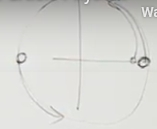
\includegraphics[width=0.6\textwidth]{two-particles-rotating}
\end{figure}

Orbital angular momentum of a point particle moving about origin. 
\begin{align*}
\vec{L} =& \vec{R} \times \vec{p} \text{ accordng to convention -- c.f. right hand rule.}\\
L_x =& y P_z - z P_y\\
L_y =& z P_x - x P_z\\
L_z =& x P_y - y P_x
\end{align*}

We will determine commutation relations of angular momentum operators.

We have \cite{susskind2014quantum}:
\begin{align*}
	[X_i,X_j] =& 0\\
	[P_i,P_j]=& 0\\
	[X_i,P_j]=& i \hslash \delta_{i,j}`
\end{align*}

\begin{thm}[Commutators for angular momentum]
	\begin{align*}
	[L_x,L_y]=& i \hslash L_z \numberthis \label{eq:lx:ly}\\
	[L_y,L_x]=& i \hslash L_x \numberthis \label{eq:ly:lz}\\
	[L_z,L_x]=& i \hslash L_y \numberthis \label{eq:lz:lx}	
	\end{align*}
\end{thm}
\begin{proof}
	\begin{align*}
	[L_x,L_y]=& [y P_z - z P_y,z P_x - x P_z]\\
	=&[y P_z, z P_x] -\cancel{[yP_z,xP_z]} -\bcancel{[zP_y,zP_x]} + [z P_y,x P_z] \\
	=& y P_x[P_z,z] + P_y x[z,P_z]\\
	=& -i \hslash y P_x + i \hslash P_y x\\
	=& i \hslash L_z \text{, which is (\ref{eq:lx:ly})} 
	\end{align*}
	The other two equations, (\ref{eq:ly:lz}) and (\ref{eq:lz:lx}) follow by cyclically permuting indices.
\end{proof}

 These relationships:
\begin{itemize}
	\item remain true if we add angular momenta for many particles;
	\item are true for spin
	 \item are relationally invariant.
\end{itemize}

We focus on the $z$-axis ("quantization axis") and introduce two new quantities--raising and lowering operators. Choosing units where $\hslash-1$:

\begin{align*}
	L_\pm \triangleq& L_x \pm i L_y \numberthis \label{eq:L_pm} \\
	[L_+,L_z] =& [Lx+i L_y,L_z]\\
	=& -iL_y + i^2 L_x \text{, from (\ref{eq:lz:lx}) and (\ref{eq:lx:ly})}\\
	=& -L_+ \text{ from (\ref{eq:L_pm}). Similarly} \numberthis \label{eq:L+:Lz}\\
	[L_-,L_z] =& + L_- \numberthis \label{eq:L-:Lz}
\end{align*}

\begin{thm}[$L_+$ is a creation operator for $L_z$]\label{thm:angular:momentum:creation}
	\begin{align*}
		L_z \ket{m} =& m \ket{m} \numberthis \label{eq:L:eigen}\\
		\implies&\\
		L_z (L_+ \ket{m}) =& (m+1) (L_+ \ket{m})
	\end{align*}	
\end{thm}

\begin{proof}
	\begin{align*}
		(\ref{eq:L+:Lz})\implies\\
		L_+L_z-L_zL_+ =& -L_+ \text{, whence:}\\
		L_zL_+ =& L_+L_z + L_+\ \text{ and}\\
		L_z L_+ \ket{m} =& (L_+L_z + L_+)\ket{m}\\
		=& L_+ (L_z + I)\ket{m}\\
		=& L_+ (m + 1) \ket{m} \text{ from (\ref{eq:L:eigen})}\\
		=&  (m + 1) (L_+ \ket{m})
	\end{align*}
\end{proof}

\begin{cor}[$L_-$ is an annihilation  operator for $L_z$]
	\begin{align*}
	L_z \ket{m} =& m \ket{m} \\
	\implies&\\
	L_z (L_- \ket{m}) =& (m-1) (L_- \ket{m})
	\end{align*}	
\end{cor}

The angular momentum spectrum is spaced by integers. How far can we bump it up before the object changes? Imagine a classical object with fixed $L^2$. We can maximize $L_z$  by pointing it upward.

Theorem \ref{thm:angular:momentum:creation} ignores the possibility that $L^+m_{max}=0$ and $L^-m_{min}=0$. (c.f. harmonic oscillator). By relational invariance, $m_{min}=-m_{max}$: Spectrum must be symmetric about zero.

There are two possibilities for the spectrum:
\begin{itemize}
	\item $-m_{max},...,-1,0,1,...m_{max}$
	\item $-m_{max},...,-\frac{1}{2},\frac{1}{2},...m_{max}$
\end{itemize}

\begin{defn}[Spin]
	$m_max$ is known as the spin. It can be 0. There are no elementary particles known with spin 3, but there are atoms. Similarly no half-spin particle over $\frac{3}{2}$.
\end{defn}

What about $L^2$? If you know $L_z$ at maximum, there will be uncertainty in other two components, so $L^2$ is not quite $m_{max}^2$.

\begin{align*}
	L_- L_+ =& (L_x-iL_y)(L_x+iL_y)\\
	=& L_x^2 +i L_x L_y -i L_y L_x + L_y^2\\
	=& L_x^2 + L_y^2 + i[L_x,L_y]\\
	=& L^2 - L_z^2 + i[Lx,Ly] \numberthis \label{eq:L-:L+}\text{, hence}\\
	L^2 =& L_- L_+ + L_z^2 \text{, classically, but this is not true for quantum world. }\\
	(\ref{eq:L-:L+}) \implies& \\
	 L^2 =& L_- L_+ + L_z^2 -\underbrace{i[Lx,Ly]}_\text{$i^2L_z$ from (\ref{eq:lx:ly})}\text{, in the quantum world}\\
	 =& L_- L_+ + L_z^2 +L_z\\
	L^2 \ket{m_{max}}=& L_- L_+ \ket{m_{max}} + L_z^2 \ket{m_{max}} +L_z \ket{m_{max}}\\
	=& (0 +m_{max}^2 + m_{max})\ket{m_{max}} \\
	=& m_{max} (m_{max}+1)\ket{m_{max}}
\end{align*}

All states have same value of $\braket{L^2}$. 

\begin{thm}[$L^2$ commutes with all its components.]
	 \begin{align*}
	 [L^2,L_i]=0  \;\forall i \in {x,y,z}
	 \end{align*}
\end{thm}
\begin{proof}
	We need the following lemma.
	\begin{lemma}[Commutator with square]\label{lemma:comm:sq}
		\begin{align*}
			[A^2,B] =& A[A,B] + [A,B]A
		\end{align*}
	\end{lemma}
	\begin{proof}[Proof of lemma]
		\begin{align*}
			[A^2,B] =& AAB - BAA\\
			=& AAB - ABA +ABA -BAA\\
			=& A[A,B] + [A,B]A
		\end{align*}
	\end{proof}
	\begin{align*}
	[L^2,L_x]=&[L_x^2,L_x] + [L_y^2,L_x] + [L_z^2,L_x] \numberthis \label{eq:L2lx}\\
	[L_y^2,L_x] =&L_y[L_y,L_x] + [L_y,L_x]L_y \text{, using Lemma \ref{lemma:comm:sq}}\\
	=& -i L_y L_z -i L_z L_y \text{ from (\ref{eq:ly:lz}). Similarly}\\
	[L_z^2,L_x] = &L_z [L_z,L_x] + [L_z,L_x] L_z\\
	=& i L_z L_y  + i L_y L_z \text{ from (\ref{eq:lz:lx}), whence (\ref{eq:L2lx}) yields}\\
	[L^2,L_x]=&\cancel{[L_x^2,L_x] }+\bcancel{ [L_y^2,L_x]} + \bcancel{[L_z^2,L_x]}
	=& 0
	\end{align*}
\end{proof}
Consider spin $\frac{1}{2}$--call them $\ket{+}$ and  $\ket{-}$.

\begin{align*}
e^{i\theta} \alpha \ket{+} + e^{i\theta}\beta \ket{-} \text{, has probability $\alpha^2$ of being in $\ket{+}$}
\end{align*}
So can ignore 1 degree of freedom. $\alpha$ and $\beta$ have 2 degrees of freedom each. Phase eliminates one, and $\alpha^2+\beta^2=1$ eliminates one other, leaving two. This is the same as number of degrees of freedom in direction.

Measured value is always $\pm \frac{1}{2}$; average may be zero; it behaves like a classical variable.

\begin{thm}[Spin statistics]
	\begin{enumerate}
		\item All particles with half integral spin are Fermions;
		\item All particles with  integral spin are Bosons.
	\end{enumerate}
\end{thm}

\begin{proof}
	TBP
\end{proof}
Take two half spin particles: composite behaves like a Boson--e.g. Hydrogen atom; deuteron is Boson, deuterium is Fermion.


\section{Spin}

\subsection{Combining Fermions to make Bosons}

Paradox: if two Fermions make a Boson, can we have two of these composite Bosons in the same state?

Wave function of Boson is supposed to be symmetric:

\begin{align*}
	\psi(x,y) =&\psi(y,x) \text{ e.g. }\\
	\psi(x,y) =& \phi(x)\phi(y)\\
	\psi(x,y) =&-\psi(y,x) \text{ for Fermions}
\end{align*}

Now imagine a wave function, $\psi(x,y)$, that isn't symmetric:
\begin{align*}
\psi(x,y)+& \psi(y,x) \text{ symmetric}\\
\psi(x,y)-& \psi(y,x) \text{ antisymmetric}
\end{align*}

Now imagine 4 Fermions--2 electons(X) and 2 protons(Y).

\begin{align*}
\psi(x_1,x_2,y_1,y_2) = &-\psi(x_2,x_1,y_1,y_2)\\
=& \psi(x_1,x_2,y_2,y_1)
\end{align*} 

Hydrogen atom at origin plus another hydrogen atom:$\psi(x_1,y_1) \phi(x_2,y_2)$.
If we antisymmetrize:
\begin{align*}
	\psi(x_1,y_1) \phi(x_2,y_2) -& \psi(x_2,y_1) \phi(x_1,y_2) 
	-\psi(x_1,y_2) \phi(x_2,y_1) + \psi(x_2,y_2) \phi(x_1,y_1)\\
	x_1 \leftrightarrow& x_2 \text{ changes sign, and}\\
	y_1 \leftrightarrow& y_2 \text{ changes sign, but}\\
	1 \leftrightarrow& 2 \text { preserves sign.}
\end{align*}

What if both atoms have same wave function? Ignoring a factor of $2$:

\begin{align*}
	\psi(x_1,y_1) \psi(x_2,y_2) -& \psi(x_2,y_1) \psi(x_1,y_2) 
\end{align*}

Both atoms can be in same place, but we can't find 2 electrons in same place.

\subsection{Mathematics of Spin}

Mathematics of Spin is needed for Colour, Isospin, etc.

\subsubsection{Half spin}

We have two values along the z axis: $S_z = m \hslash$. We will use $S$ for spin, $L$ for orbital angular momentum.

\begin{align*}
	[S_x,S_y] =& i S_z \numberthis \label{eq:sx:sy}\\
	[S_y,S_z] =& i S_x  \numberthis \label{eq:sy:sz}\\
	[S_z,S_x] =& i S_y  \numberthis \label{eq:sz:sx}\\
	S_\pm =& S_x \pm S_y
\end{align*}
Compare with (\ref{eq:lx:ly}),  (\ref{eq:ly:lz}), and  (\ref{eq:lz:lx}).

Can express spin as $\begin{pmatrix}
\alpha\\
\beta
\end{pmatrix}$ or $\alpha\ket{+} + \beta\ket{-}$ 

Components are 2D matrices satisfying algebra (\ref{eq:sx:sy}), (\ref{eq:sy:sz}), and (\ref{eq:sz:sx}). They are not unique, but equivalent. We will use the Pauli spin\footnote{Without $\frac{1}{2}$ they are known as Pauli matrices.}:
\begin{align*}
	S_x =& \frac{1}{2}\begin{pmatrix} \numberthis \label{eq:pauli:x}
		0&1\\
		1&0
	\end{pmatrix}\\
	S_y =& \frac{1}{2}\begin{pmatrix} \numberthis \label{eq:pauli:y}
		0&-i\\
		i&0
	\end{pmatrix}\\
	S_z =& \frac{1}{2}\begin{pmatrix} \numberthis \label{eq:pauli:z}
		1&0\\
		0&-1
	\end{pmatrix}
\end{align*}

\subsubsection{Spin 1}

We have three states $\{-1,0,1\}$, a Boson. Are there $3\times3$ matrices satisfying (\ref{eq:sx:sy}), (\ref{eq:sy:sz}), and (\ref{eq:sz:sx})?

\begin{align*}
	S_z = i \begin{pmatrix}
		0&1&0\\
		-1&0&0\\
		0&0&0
	\end{pmatrix}\\
	S_y = i \begin{pmatrix}
		0&0&1\\
		0&0&0\\
		-1&0&0
	\end{pmatrix}\\
	S_x = i \begin{pmatrix}
		0&0&0\\
		0&0&1\\
		0&-1&0
	\end{pmatrix}
\end{align*}

Find eigenstates of $S_z$:
\begin{align*}
	i \begin{pmatrix}
		0&1&0\\
		-1&0&0\\
		0&0&0
	\end{pmatrix}\begin{pmatrix}
		\alpha\\
		\beta\\
		\gamma
	\end{pmatrix}=&\begin{pmatrix}
		\alpha\\
		\beta\\
		\gamma
	\end{pmatrix}\\
	=&i\begin{pmatrix}
		\beta\\
		-\alpha\\
		0
	\end{pmatrix}
\end{align*}

Return to real electron that can move in space. We turn the 2D spinors into functions of position: $\begin{pmatrix}
\psi_u(x)\\
\psi_d(x)
\end{pmatrix}$.

For spin 1: $\begin{pmatrix}
\phi_1(x)\\
\phi_2(x)\\
\phi_3(x)
\end{pmatrix}$.

\subsection{Dirac Equation: connection with Spin}

\begin{align*}
i \frac{\partial \psi}{\partial t} =& - i \alpha_i \frac{\partial \psi}{\partial x^i} + \beta m \psi\\
\omega =& \sum_i \alpha_i k_i + \beta m\\
\omega^2 =& k^2 + m^2
\end{align*}
Where the $\alpha_i$ and $\beta$ satisfy (\ref{eq:dirac:ac1}), (\ref{eq:dirac:ac2}), (\ref{eq:dirac:ac3}), and (\ref{eq:dirac:ac4}).


\begin{thm}[Dirac anticommutation relations.]\label{thm:dirac:anticommutation} 
	Equations (\ref{eq:dirac:ac1}), (\ref{eq:dirac:ac2}), (\ref{eq:dirac:ac3}), and (\ref{eq:dirac:ac4}) can be satisfied by suitably chosen $2\times4$ matrices, and they cannot be satisfied by $n \times n$ for $n<4$.
\end{thm}
\begin{proof}
	TBP
\end{proof}

One set of solutions, which is not the same as (\ref{eq:beta:1}), (\ref{eq:alpha1:1}), (\ref{eq:alpha2:1}), and (\ref{eq:alpha3:1}):
\begin{align*}
	\alpha_i=&\begin{pmatrix}
		\sigma_i&0\\
		0&-\sigma_i
	\end{pmatrix}\\
	\beta =& \begin{pmatrix}
		0&I\\
		I&0
	\end{pmatrix}
\end{align*}

There are two kinds of $2\times2$: 2 blocks of $2\times2$ matrices. This corresponds to the physics - there are two energies, positive and negative, and two spins.
The 4 components are not a relativistic 4-vector! The easiest way to see this is to set momentum to zero, then the $\alpha_i$ drop out.

\begin{align*}
i \frac{\partial \psi}{\partial t} =&  \beta m \psi \text{ for particle at rest.}\\
i \frac{\partial}{\partial t}\begin{pmatrix}
\psi_+\\
\psi_-
\end{pmatrix}=&m \begin{pmatrix}
0&I\\
I&0
\end{pmatrix}\begin{pmatrix}
\psi_+\\
\psi_-
\end{pmatrix}\\
i \frac{\partial \psi_+}{\partial t} =&   m \psi_-\\
i \frac{\partial \psi_-}{\partial t} =&   m \psi_+ \\
i \frac{\partial (\psi_++\psi_-)}{\partial t} =&   m (\psi_++\psi_-) \text{ positive energy--$\omega=m$}\\
i \frac{\partial (\psi_+-\psi_-)}{\partial t} =&   -m (\psi_+-\psi_-) \text{ negative energy--$\omega=-m$}
\end{align*}

So we end up with two uncoupled equations! $2\times2$ is connected to positive and negative energies. $2\times2$ of $\psi_+$ arises from spin.


\section{Equations of motion of particles and fields}\label{sect:equation:motion}

The equations of motion of fields that describe  particles all come from a Lagrangian. In quantum field theory, Lagrangian describes everything.

\subsection{Review of classical fields}

\begin{align*}
\mathcal{L}=& \mathcal{L}(\phi,\partial_t \phi, \partial_x \phi)\\
=&\mathcal{L}(\phi,\partial_{\mu} \phi) \text{ in Minkowski space}\\
\frac{\partial}{\partial t} \frac{\partial \mathcal{L}}{\partial \big(\frac{\partial \phi}{\partial t}\big)}+\sum_i \frac{\partial}{\partial x_i} \frac{\partial \mathcal{L}}{\partial \big(\frac{\partial \phi}{\partial x_i}\big)}=&\frac{\partial \mathcal{L}}{\partial \phi} \text{, equation of motion} \numberthis \label{eq:lagrange}
\end{align*}

(If $\mathcal{L}$ depends on several fields, there will be a version of (\ref{eq:lagrange})  for each field.)

Example of $\mathcal{L}$.

\begin{align*}
	\mathcal{L} =& \frac{1}{2} (\frac{\partial \phi}{\partial t})^2 - \frac{1}{2} (\frac{\partial \phi}{\partial x})^2 - \frac{1}{2} (\frac{\partial \phi}{\partial y})^2 - \frac{1}{2} (\frac{\partial \phi}{\partial z})^2 - V(\phi)
\end{align*}

Substituting in (\ref{eq:lagrange}):
\begin{align*}
	\ddot{\phi} - \frac{\partial^2 \phi}{\partial x^2}  - \frac{\partial^2 \phi}{\partial y^2}  - \frac{\partial^2 \phi}{\partial z^2} =& - \frac{\partial V}{\partial \phi} \text{. The simplest interesting case is:}\\
	V(\phi) =& \frac{m^2 \phi^2}{2}\\
	\ddot{\phi} - \frac{\partial^2 \phi}{\partial x^2}  - \frac{\partial^2 \phi}{\partial y^2}  - \frac{\partial^2 \phi}{\partial z^2} =& - m^2 \phi \numberthis \label{eq:simplest:non:trivial}
\end{align*}

Differentiating a wave function $e^{-i \omega t} e^{-i k x}$ twice by $t$ gives a factor $-\omega^2$. Substituting in (\ref{eq:simplest:non:trivial}):
\begin{align*}
-\omega^2 \cancel{\phi} - (k_x^2+k_y^2+k_z^2)\cancel{\phi} =& -m^2 \cancel{\phi}\\
-\omega^2  - (k_x^2+k_y^2+k_z^2) =& -m^2 \\
\omega^2 + P^2 = m^2
\end{align*}

If $\mathcal{L}$ is a scalar, equations of momentum will be Lorentz Invariant.

What about a more complex $V(\phi)$?
\begin{align*}
	V(\phi) =& \frac{m^2 \phi^2}{2} + g \phi^3\\
	\ddot{\phi} - \frac{\partial^2 \phi}{\partial x^2}  =& - m^2 \phi - 3 g \phi^2
\end{align*}

Quadratic terms in Lagrangian lead to linear equations; higher powers lead to non-linearities, so cannot superpose. May scatter.

Consider two fields:
\begin{align*}
	\mathcal{L} =& \frac{1}{2}(\partial_{\mu} \phi)^2 + \frac{1}{2}(\partial_{\mu} \rho)^2 - \frac{m^2 \phi^2}{2} - \frac{M^2 \rho^2}{2} - \rho \phi^2\\
	\ddot{\phi} - \partial_x^2 \phi =& -m^2 \phi - \rho \phi
	\\
	\ddot{\rho} - \partial_x^2 \rho =& -m^2 \rho -phi^2
\end{align*}

These are non-linear and coupled, so the particles scatter each other.

Consider the Dirac equation.

\begin{align*}
\dot{\psi} =& i \alpha \frac{\partial \psi}{\partial x} + m \beta \psi\\
\mathcal{L} =& i \big( \psi^\dagger \partial_t \psi +  \psi^\dagger \alpha \partial_x \psi + \psi^\dagger \beta \psi m \big)
\end{align*}

Suppose there is another field: can add scalar field to Dirac field and get scattering, and generate equations of motion for both fields.

\begin{align*}
\mathcal{L} =& i \big( \psi^\dagger \partial_t \psi +  \psi^\dagger \alpha \partial_x \psi + \psi^\dagger \beta \psi m \big) - \psi^\dagger \beta \psi \phi
\end{align*}

Lagrangian is what specifies a field theory.

\subsection{Quantum Fields}

Imagine Lagrangian containing $\phi^3$, where $\phi = (a_+ + a_-)$.
Figure \ref{fig:phi:3:x} shows the kinds of interaction that may occur. Quadratic terms in Lagrangian give rise to motion, higher powers to interactions: 1 particle $\rightarrow$ 2, 2 particles $\rightarrow$ 1, 0 particles $\rightarrow$ 3, 3 particles $\rightarrow$ 0.
 
\begin{figure}[H]
	\caption{$\phi^3(x)$ gives rise to many possible interactions.}\label{fig:phi:3:x}
	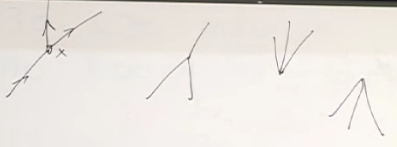
\includegraphics[width=0.8\textwidth]{phi-3-x}
\end{figure}

How to change position of particle. We need a pair of operators $\phi(x) \phi(x^\prime)$ to absorb particle at $x$, and re-emit at $x^\prime$--i.e. move particle

\begin{align*}
(\frac{\partial \phi}{\partial x})^2 =& \frac{\big( \phi(x) - \phi(x^\prime)\big)^2}{...}\\
=& \frac{\phi(x)^2 + \phi(x^\prime)^2 - 2  \phi(x) \phi(x^\prime)}{...}
\end{align*}

Electromagnetic field and Dirac electron.

\begin{align*}
	\psi =& c_e^-(\text{+ve energy}) + c_e^-(\text{+ve energy}) \text{ Dirac field}\\
	\psi =& c_e^-(\text{+ve energy}) + c_p^+(\text{+ve energy}) \text { Dirac sea--$p$ for positron}\\
	\psi^\dagger =& c_e^+(\text{+ve energy}) + c_e^+(\text{+ve energy})\\
	=& c_e^+(\text{+ve energy}) + c_p^-(\text{+ve energy})
\end{align*}

Basic interaction of electrodynamics.
\begin{align*}
	e \big( \psi^\dagger \psi A_0 + 	\underbrace{\psi^\dagger \alpha_i  \psi}_\text{vector from $\psi$} A_i \big) \text{ polarization of photon $A$} \numberthis \label{eq:basic:interaction}
\end{align*}

\begin{figure}[H]
	\caption{Interactions arising from Lagrangian (\ref{eq:basic:interaction})}
	\begin{subfigure}{0.48\textwidth}
		\caption{Annihilation + 2 creation: photon emitted}
		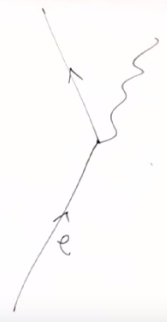
\includegraphics[width=0.7\textwidth]{em-dirac1}
	\end{subfigure}
	\begin{subfigure}{0.48\textwidth}
		\caption{2 Annihilation +  creation: photon absorbed}
		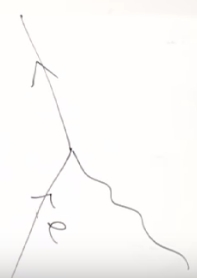
\includegraphics[width=0.7\textwidth]{em-dirac2}
	\end{subfigure}
	\begin{subfigure}{0.48\textwidth}
		\caption{2 Annihilation +  creation: Electron + positron produces photon. NB, by convetion, positron is drawn with downward arrow.}
		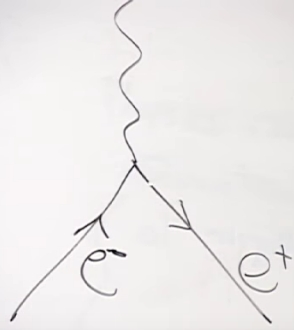
\includegraphics[width=0.7\textwidth]{em-dirac3}
	\end{subfigure}
	\begin{subfigure}{0.48\textwidth}
		\caption{Photon absorbed, electron and positron created.}
		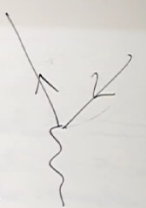
\includegraphics[width=0.7\textwidth]{em-dirac4}
	\end{subfigure}
	\begin{subfigure}{0.48\textwidth}
		\caption{Photon, electron and positron absorbed (energy and momentum not conserved!).}\label{fig:em:dirac5}
		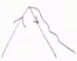
\includegraphics[width=0.7\textwidth]{em-dirac5}
	\end{subfigure}
\end{figure}

$e$ is strength of interaction, probability of interaction $e^2$.

Remember that energy conservation arose from integrating over all time, and momentum conservation from integrating over space. If we integrate (\ref{eq:basic:interaction}) over all space and all time,  energy and momentum will both be conserved, which rules out the process depicted in Figure \ref{fig:em:dirac5}.

Protons, Neutrons, Pi mesons. Pions are scalar particles, and they come in 3 types, $\pi_+$, $\pi_-$, $\pi_0$.

\begin{table}[H]
	\begin{center}
		\caption{Protons, Neutrons, Pi mesons}
		\begin{tabular}{|l|l|} \hline
			Operators &Description\\ \hline
			$\psi_p$, $\psi^\dagger_p$& create and annihilate proton\\ \hline
		    $\psi_n$, $\psi^\dagger_n$& create and annihilate neutron\\ \hline
			$\pi_+$& annihilate pion\\ \hline
			$\pi_-$&annihilate pion\\ \hline
			$\pi_0$&annihilate pion\\ \hline
			$\psi^\dagger_p \psi_n \pi_+$&Absorb pion and neutron, emit proton\\ \hline
			$\psi^\dagger_n \psi_p \pi_-$&Absorb pion and proton, emit neutron\\ \hline
			$\psi^\dagger_p \psi_p \pi_0$&Absorb pion and proton, emit proton\\ \hline
			$\psi^\dagger_n \psi_n \pi_0$&Absorb pion and neutron, emit neutron \\ \hline
		\end{tabular}
	\end{center}
\end{table}
The fundamental process of course involve quarks; if energy is high enough to break up protons, cannot use proton fields..

\begin{figure}[H]
	\caption{Two processes from the same interaction.}
	\begin{subfigure}{0.45\textwidth}
		\caption{Proton $\rightarrow$ neutron + pion}
		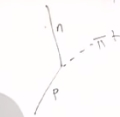
\includegraphics[width=0.8\textwidth]{pion1}
	\end{subfigure}
	\begin{subfigure}{0.45\textwidth}
		\caption{Proton + antineutron $\rightarrow$ pion}
		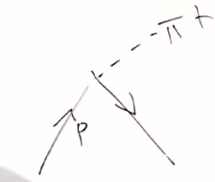
\includegraphics[width=0.8\textwidth]{pion2}
	\end{subfigure}
\end{figure}

The Lagrangian describes things that happen at a point, or a pair of neighbouring points. Figure \ref{fig:proton:electron:photon} shows an interaction arising from a product of terms. There is no action at a distance.
\begin{figure}[H]
	\caption[Proton photon electron interaction]{Proton photon electron interaction--product of two separate terms in Lagrangian}\label{fig:proton:electron:photon}
	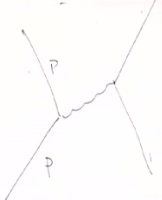
\includegraphics[width=0.8\textwidth]{proton-electron-photon}
\end{figure}

NB: creation operators are functions of P or X, never both (uncertainty principle). They are related through Fourier transforms, which are the essence of the uncertainty principle.

$\bra{0}\psi^\dagger\psi^\dagger\psi^\dagger...\mathcal{L}\mathcal{L}\mathcal{L}...\psi\psi\psi\ket{0}$

\begin{align*}
	\Pi_i& \big(1+\mathcal{L}_{interaction}(x_i)\big)\\
	=&1 + \sum_i \underbrace{ \mathcal{L}(x_i)}_\text{one vertex}  +\sum_{i,j}\underbrace{\mathcal{L}(x_i)\mathcal{L}(x_j)}_\text{two vertices} +...
\end{align*}

We get an infinite number of places where 1 thing, 2 things, etc, happen.

The art form is figuring out the Lagrangian; then \gls{gls:QFT} becomes a precise tool.

Often can ignore parts of Lagrangian: e.g. quarks don't have much to do with electrons. QFT may be a coarse grained description of something else.
 

\section{Field Lagrangians and Path Integrals}

The basic technique that Lecture \ref{sect:equation:motion} alluded to is called the \emph{path integral method of quantum mechanics}. It is the most direct route to the theory of particle interactions based on Feynman diagrams. The path integral is the quantum mechanical version of the Principle of Least Action\cite{susskind2013quantum}. If we think of a classical Newtonian particle, its motion from one point of space-time to another is determined by a Lagrangian $\mathcal{L}(\dot{X},X)$. We use the Lagrangian to construct the Action. 

\begin{defn}[Classical Action of Path]
	For every trajectory, $P$ from the initial point to the final point, whether or not the trajectory is a solution to Newton's Laws of motion,  the Classical Action is: 
	\begin{align*}
		\mathcal{A}=\int_P dt \mathcal{L}(\dot{X},X)
	\end{align*}
\end{defn}


The classical form of the Principle of Least Action is that the true trajectory minimizes the action. We can use the calculus of variations to derive differential equations which satisfy Newton's Laws. The same idea works in classical field theory, where $\mathcal{L}=\mathcal{L}(\phi,\partial_\mu\phi)$. The theory of relativity requires that the Lagrangian be a scalar\cite{susskind2017special}.

\begin{defn}[Action over Region]
	For a region of spaces time, $R$,  the Action is: 
	\begin{align*}
		\mathcal{A}=\int_R dx^4 \mathcal{L}(\phi,\partial_\mu\phi)
	\end{align*}
\end{defn}

The analogue of the starting point for a particle is the initial value of the field. If we prescribe the starting and final values of the field, we can ask whether there is a solution that starts with starting values, and ask whether there is a solution that minimizes the action. The principle of least action states that the correct value of the field is the one that minimizes the action. So the original principal of least action gets extended to a space-time principal of least action, where the degrees of freedom are fields. NB, we are looking for a way to interpolate the field which minimizes the Action.
\url{https://youtu.be/q-QaaKCvDUs?t=555}
We now look at the quantum mechanical use of Action: \emph{we won't attempt to derive the classical version from the quantum mechanical version.}

According to quantum mechanics, a thing that you might want to calculate is the \emph{amplitude}, so we can calculate probabilities. Imagine that particle is injected at $(x,t)$: what is amplitude that particle will be found at $(x^\prime,t^\prime)$?

Feynman's rule is:

\begin{align*}
	Amplitude =& \sum_{Histories} e^{-\frac{i}{\hslash} \int \mathcal{L} dt}
\end{align*}

where the sum is taken over all classically \emph{possible} histories--Figure \ref{fig:sum:histories}--i.e. they can not go back in time for non-relativistic QM. Probability is the square of the magnitude of the Amplitude.

\begin{figure}[H]
	\caption{Sum over histories}\label{fig:sum:histories}
	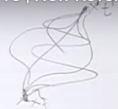
\includegraphics[width=0.8\textwidth]{sum-histories}
\end{figure}



Imagine starting systems with field $\phi(x)$, and asking for probability of $\phi^\prime(x)$ at some later time--Figure \ref{fig:path-integral1}. Again this is determined by an amplitude:
\begin{align*}
	\sum e^{-\frac{i}{\hslash} \int dx dy dz dt\mathcal{L}(\phi,\partial \phi) }
\end{align*}
summed over all possible histories between $\phi(x)$ and $\phi^\prime(x)$.

\begin{figure}[H]
	\caption{Initial and final conditions}\label{fig:path-integral1}
	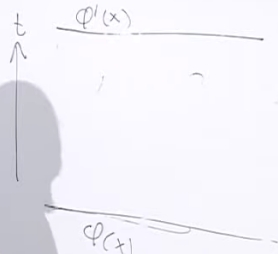
\includegraphics[width=0.8\textwidth]{path-integral1}
\end{figure}

(A question was asked about convergence: trajectories tend to cancel, and those with the least cancellation tend to be near the ones that have least action classically.)

There are two ways to think of quantum field theory, in terms of fields, and in terms of particles. What if we specify field quanta (particles)? We ask the probability of some specified particle content at a later time. The answer involves a path integral. Start by partitioning space into cells--Figure \ref{fig:path-integral2}--and think about the value of the field in each cell. We compute:
\begin{align*}
	\Pi_{i\in cells}(1-\frac{i}{\hslash} \mathcal{L_i}a^4) \text{, where $a^4$ is volume of a cell.}
\end{align*}
 
Now we have the following approximation for small $\epsilon$
\begin{align*}
	1 + \epsilon \approx &e^\epsilon\\
	\approx& 1 + \frac{\epsilon}{1!} + \frac{\epsilon^2}{2!}  + \frac{\epsilon^3}{3!} +...\\
\end{align*}

\begin{align*}
	\sum_{histories} e^{-\frac{i}{\hslash} \int dx dy dz dt\mathcal{L}(\phi,\partial \phi) } =& \sum_{histories} e^{-\frac{i}{\hslash} A_i } \text{, where $A_i$ is action in $i$th cell}\\
	=& \sum_{histories} \Pi_i e^{-\frac{i}{\hslash} A_i }
\end{align*}

Let's forget particles for a moment and think of fields.

\begin{figure}[H]
	\caption[Space partitioned into cells]{Space partitioned into cells. Initial conditions in bottom row, final in top. We consider all possible histories that match initial and final conditions. NB: functions aren't necessarily analytic or even continuous.}\label{fig:path-integral2}
	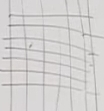
\includegraphics[width=0.8\textwidth]{path-integral2}
\end{figure}

Our question is now: if initial condition matches our initial configuration of particles, and final condition matches desired configuration, what is the amplitude? Figure \ref{fig:path-integral3} depicts a particle moving in one history.

\begin{figure}[H]
	\caption[Particle moving]{Creation operator in one cell, annihilation in neighbour amounts to movement}\label{fig:path-integral3}
	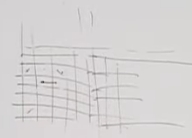
\includegraphics[width=0.8\textwidth]{path-integral3}
\end{figure}

There are terms in the Lagrangian associated with pairs of boxes--the derivatives:
\begin{align*}
	\frac{1}{2}(\partial_t \phi)^2 \rightarrow& \frac{1}{2}\frac{(\phi(t,x)-\phi(t^\prime,x))^2}{...}\\
	\frac{1}{2}(\partial_x \phi)^2 \rightarrow& \frac{1}{2}\frac{(\phi(t,x)-\phi(t,x^\prime))^2}{...} \numberthis \label{eq:phi:phi}
\end{align*}
(\ref{eq:phi:phi}) gives rise to terms such as:
\begin{alignat*}{2}
	e^{- i \sum_{neighbours} \phi(x) \phi(x^\prime)}=1& -&& i \sum_{neighbours} \underbrace{\phi(x) \phi(x^\prime)}_\text{Figure \ref{fig:path-integral5}}\\
&-&& \frac{1}{2!}\underbrace{\sum_{neighbours} \phi(x) \phi(x^\prime)\sum_{neighbours} \phi(x^{\prime\prime}) \phi(x^{\prime\prime\prime})}_\text{Figure \ref{fig:path-integral7}}\\
&+&&\underbrace{i\frac{1}{3!}\sum_{neighbours}\phi(..)\phi(..)\sum_{neighbours}\phi(..)\phi(..)\sum_{neighbours}\phi(..)\phi(..)}_\text{Figure \ref{fig:path-integral9}}\\
&+&& ... \numberthis \label{eq:path:integral:expanded}
\end{alignat*}



\begin{figure}[H]
	\caption{Rules for Path Integrals}
	\begin{subfigure}{0.45\textwidth}
		\caption{Create at one point, annihilate at neighbour}\label{fig:path-integral5}
		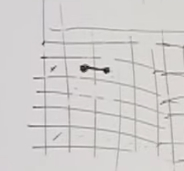
\includegraphics[width=1.0\textwidth]{path-integral5}
	\end{subfigure}
	\begin{subfigure}{0.45\textwidth}
		\caption{A dangling endpoint is illegal unless one endpoint creates, other annihilates: since we are only putting particles in from initial state and removing from final, this is illegal.}\label{fig:path-integral4}
		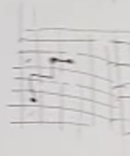
\includegraphics[width=1.0\textwidth]{path-integral4}
	\end{subfigure}
	\begin{subfigure}{0.45\textwidth}
		\caption{The only way Figure \ref{fig:path-integral5} can contribute is if space is only two layers thick.}\label{fig:path-integral6}
		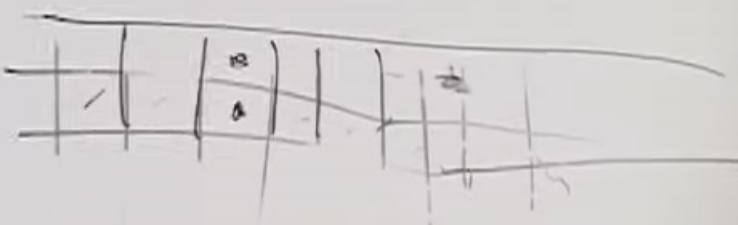
\includegraphics[width=1.0\textwidth]{path-integral6}
	\end{subfigure}
	\begin{subfigure}{0.45\textwidth}
		\caption{What about thicker space? How to we get from \ref{fig:path-integral6} to here? We need the quadratic term in (\ref{eq:path:integral:expanded})}\label{fig:path-integral7}
		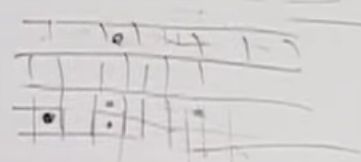
\includegraphics[width=1.0\textwidth]{path-integral7}
	\end{subfigure}
	\begin{subfigure}{0.45\textwidth}
		\caption{How to avoid dangling ends in \ref{fig:path-integral7}? Restrict to 3 layers. This allows us to find $x^\prime=x^{\prime\prime}$ in (\ref{eq:path:integral:expanded})}\label{fig:path-integral8}
		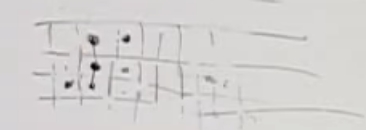
\includegraphics[width=1.0\textwidth]{path-integral8}
	\end{subfigure}
	\begin{subfigure}{0.45\textwidth}
		\caption{Including the cubic term in (\ref{eq:path:integral:expanded}) allows us to find two 3-step paths in (\ref{eq:path:integral:expanded}).}\label{fig:path-integral9}
		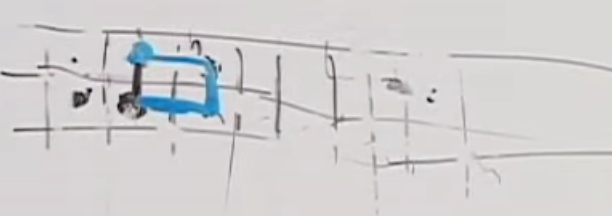
\includegraphics[width=1.0\textwidth]{path-integral9}
	\end{subfigure}
\end{figure}

So we can sum up contributions $\frac{i^n}{n !}$ in (\ref{eq:path:integral:expanded}) to determine complex amplitude. We include backward paths from special relativity--Figure \ref{fig:path:backward:time}.

\begin{figure}[H]
	\caption{Path going backwards in Time. We can think of it in two ways.}\label{fig:path:backward:time}
	\begin{subfigure}{0.45\textwidth}
		\caption{New rule allows particle to go back in time}
		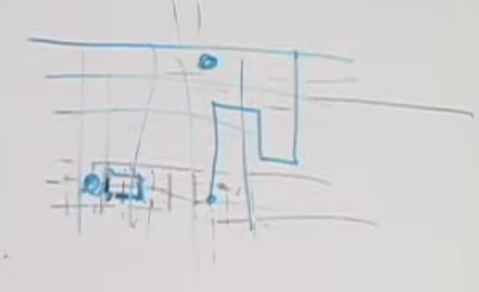
\includegraphics[width=0.8\textwidth]{path-backward-time}
	\end{subfigure}
	\begin{subfigure}{0.45\textwidth}
		\caption{Particle anti-particle pair used instead.}
		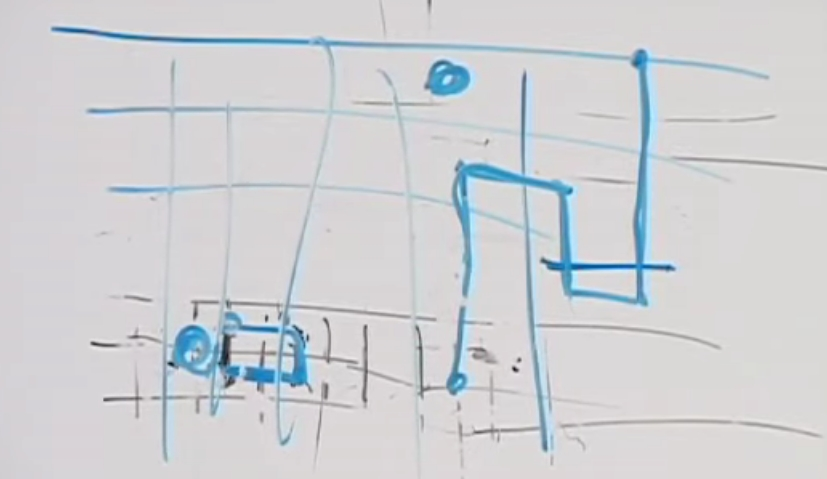
\includegraphics[width=0.8\textwidth]{path-backward-time1}
	\end{subfigure}
\end{figure}

Two particles.

\begin{figure}[H]
	\caption{Two particles}\label{fig:path:integral:2particles:1}
	\begin{subfigure}{0.45\textwidth}
		\caption{Quadratic term in (\ref{eq:path:integral:expanded}) used to advance two particles by one box}
		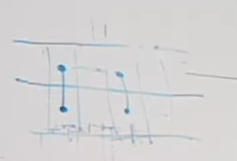
\includegraphics[width=0.8\textwidth]{path-integral-2particles-1}
	\end{subfigure}
	\begin{subfigure}{0.45\textwidth}
		\caption{Weight particle by $m^2$ from $\frac{m}{2}\phi^2$}\label{fig:path:integral:mass}
		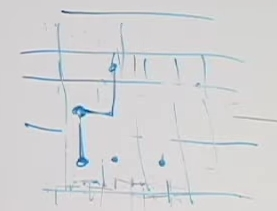
\includegraphics[width=0.8\textwidth]{path-integral-mass}
	\end{subfigure}
\end{figure}

What goes in Lagrangian?

\begin{align*}
\mathcal{L}=& \frac{1}{2} (\partial_t \phi)^2 - \frac{1}{2} (\partial_x \phi)^2 + \underbrace{\frac{m}{2}\phi^2}_\text{ absorb and emit at same point} +\underbrace{g \phi^3}_\text{Figure \ref{fig:path:integral:cubic}}
\end{align*}

This weights path by $m^2$--Figure \ref{fig:path:integral:mass}. If not used we have theory of massless particles.

\begin{figure}[H]
	\caption{Some possibilities from $\phi^3$}
	\begin{subfigure}{0.4\textwidth}
	\caption{Particle absorbed and two new particles created.}\label{fig:path:integral:cubic}
		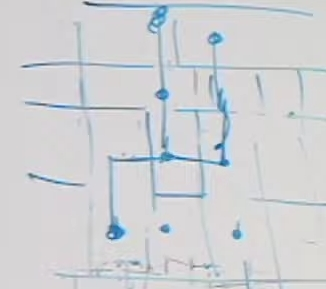
\includegraphics[width=0.8\textwidth]{path-integral-cubic}
	\end{subfigure}
	\begin{subfigure}{0.4\textwidth}
		\caption{Particle emitted and later reabsorbed.}\label{fig:path:integral:cubic:split}
		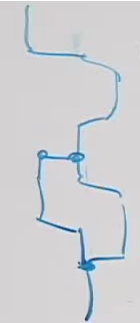
\includegraphics[width=0.8\textwidth]{path-integral-cubic-split}
	\end{subfigure}
	\begin{subfigure}{0.4\textwidth}
		\caption{Electron emits and absorbs photon.}\label{fig:path:integral:cubic:split1}
		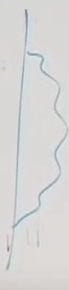
\includegraphics[width=0.5\textwidth]{path-integral-cubic-split1}
	\end{subfigure}
	\begin{subfigure}{0.4\textwidth}
		\caption{More complex version of Figure \ref{fig:path:integral:cubic:split1}.}\label{fig:path:integral:cubic:split2}
		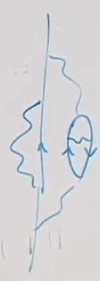
\includegraphics[width=0.5\textwidth]{path-integral-cubic-split2}
	\end{subfigure}
\end{figure}

How come answer not infinite? Powers of coefficients from Lagrangian $(g)$ appear with different powers; hope they are small enough.

Feynman diagrams and Lagrangians are complementary.

% glossary: may need command makeglossaries particles1
\printglossaries

\bibliographystyle{unsrt}
\addcontentsline{toc}{section}{Bibliography}
\bibliography{tm}

\end{document}
